\section{Основне особине сигнала и система}
\subsection{Континуални и дискретни сигнали}

\refstepcounter{ID}
\setcounter{fid}{0}
\graphicspath{{./1_uvod/1_osnovne_osobine_signala/}}
\noindent
%\vspace{-10mm}
\subsubsection{\textit{Делта импулс и хевисајднова одскочна функција}}
\noindent
\textbf{\ID}. 
Скицирати временски дијаграм сигнала датог изразом $x(t) = \updelta(f(t))$ где је 
$f(t) = t^2 - 1$, а
$\updelta(t)$ Дираков импулс. \\[2mm]

\textsc{\underline{Решење}}: 

\begin{slikaDesno}
[1]
[$t^2 - 1$ (- - -), $\updelta(t^2 - 1)$ (---)]
{fig/dirac_pm1.pdf}
Користећи дефинициону особину Дираковог импулса да је $\updelta(t \neq 0) = 0$, 
закључујемо да је $x(t) = 0$ за $f(t) \neq 0$. На основу тога, ненулту вредност ће дати сигнал имати 
само у тачкама које су решење једначине $f(t) = t^2 - 1 = 0$ односно $t = \pm 1$.  
Даље, приметимо да је за даљу анализу релевантна само непосредна околина 
тачака $t = \pm 1$, односно, једино је релевантно колико „брзо“ сигнал пролази
кроз нулу -- за шта је мера први извод у тој тачки. Одређивањем извода  има се да је 
$\dfrac{\de f(t)}{\de t} = 2t = \pm 2$ за $t = \pm 1$. 
\end{slikaDesno}
Користећи особину да је $\updelta( k(t - \uptau) ) = \dfrac{1}{|k|} \updelta(t - \uptau)$, онда 
се може писати 
${x(t) = \dfrac12 \updelta(t - 1) + \dfrac12 \updelta(t + 1)}$. Добијени резулат илустрован је на слици 
\ID.1. 
\vspace*{\ProblemSep}

\refstepcounter{ID}
\setcounter{fid}{0}
\graphicspath{{./1_uvod/1_osnovne_osobine_signala/}}
\noindent

\begin{slikaDesno}[1][]{fig/delta_povorka_pi.pdf}
\PID Континуални сигнал $\updelta(\sin(t))$ расписати преко скалираних и померених 
Делта импулса и скицирати његов временски дијаграм. \\[5mm]
\textsc{\underline{Резултат}}: Сигнал се може изразити као поворка Диракових импулса у облику 
${x(t) = {\DS \sum_{k = -\infty}^{\infty} \updelta(t - k\uppi)}} = 
\text{Ш}_\uppi(t)$.  Traжена скица приказана је 
на
слици \ID.1. 
\end{slikaDesno}

\vspace*{\ProblemSep}

\refstepcounter{ID}
\setcounter{fid}{0}
\graphicspath{{./1_uvod/1_osnovne_osobine_signala/}}
\noindent
\noindent
\begin{slikaDesno}[0.833]{fig/C.pdf}\noindent
\textbf{\ID}. \label{ID:capID}
У колу са слике познато је 
$C = 1 \unit{\upmu F}$. 
Идеалан прекидач П је отворен, а кондензатор је оптерећен количином
наелектрисања $Q = 1 \unit{\upmu C}$. У тренутку $t_0 = 0$ затвара се прекидач. 
Одредити $v_{C} = v_{C}(t)$        
и $i_{\Uppi} = i_{\Uppi}(t)$, за $-\infty < t < \infty$. 
\end{slikaDesno}

\textsc{\underline{Решење}}.
Према услову задатка је 
\vspace{1mm}
$v_C(t < 0) = \dfrac{Q}{C} = 1\unit{V}$. Према карактеристици идеалног прекидача
након затварања прекидача је $v_C(t > 0) = 0$, обједињено ово се може записати у условном облику као 
$
v_C(t) = 
\begin{cases}
        1\unit{V},&  t < 0 \\
        0,        &  t > 0
\end{cases}.
$ Добијени израз се може записати и помоћу Хевисајдове одскочне функције као 
\begin{equation}
v_{\rm C} = 1\unit{V} ( 1 - \uu(t) ). 
\end{equation}
Тако записан израз је нарочито користан за одређивање тражене струје, пошто је струја кондензатора, 
за референтни смер услклађен са напоном, 
константне капацитивности дата изразом $i_C = C\dfrac{\de v_C}{\de t}$, она се може потражити као
$
i_C = \dfrac{\de v_{\rm C}}{\de t} = - 1\unit{\upmu C} \dfrac{\de \uu(t)}{\de t}  = 
- 1\unit{\upmu C} \, \updelta(t). 
$
Пошто је добијена струја кондензаора у супротном референтном смеру од струје прекидача, коначан 
резултат за струју прекидача је 
$i_{\Uppi}(t) = 1\unit{\upmu C} \, \updelta(t)$.

Важно је прокоментарисати две ствари у вези са овим резултатом. Прво, физички смисао Делта импулса може
се потражити у свим појавама које трају веома кратко а које имају коначан утицај. У овом случају, 
за „бесконачно кратко“ време кроз прекидач протекне целокупно наелектрисање кондензатора. Са друге 
стране, приметимо да је димензија сигнала $\delta(t)$ заправо $\unit{s^{-1}}$, па је мера делта импулса
који одговара струји заправо количина наелектрисања. Ово је конзистентно са дефиниционим својством
Дираковог импулса према $\DS \int_{-\infty}^{\infty} 
\underbrace{\updelta(t)}_{\unit{s^{-1}}} \, 
\underbrace{\de t}_{\unit s} = \underbrace{1}_{[\cdot]}$.
\vspace*{\ProblemSep}

\refstepcounter{ID}
\setcounter{fid}{0}
\graphicspath{{./1_uvod/1_osnovne_osobine_signala/}}
\noindent
\textbf{\ID.} 
Нека је дат
континуалан сигнал
$
\DS x(t) = {\rm e}^{\upsigma t} \,
%\sum_{k = -\infty}^\infty \updelta(t - kT)$ 
\text{Ш}_T(t)
\,\uu(t + \upepsilon)$, где је  $0 < \upepsilon < T$.
(а) Одредити услов које треба да задовољава параметар $\upsigma\in\mathbb R$ тако да интеграл
$\DS \int_{-\infty}^{\infty} \hspace*{-0.5em} x(t)\,\de t$ конвергира, 
и у том случају (б) израчунати  тај интеграл.
\vspace{5mm}

\textsc{\underline{Решење}}: (а) Дата поворка Делта импулса се може расписати по дефиницији, а 
затим се може применити особина еквиваленције\footnote{Особина \textit{еквиваленције} је 
$x(t) \updelta(t - t_0) = x(t_0) \updelta(x - t_0)$. } Делта импулса према
\begin{equation}
    x(t) = {\rm e}^{\upsigma t} \,
    \underbrace{ \sum_{k = -\infty}^\infty \updelta(t - kT) }_{\text{Ш}_T(t)}
    \,\uu(t + \upepsilon) = 
    \sum_{k = -\infty}^\infty \underbrace{ {\rm e}^{\upsigma t} \updelta(t - kT) }_{\text{особина екв.}}
    \,\uu(t + \upepsilon)
    =
    \sum_{k = -\infty}^\infty {\rm e}^{\upsigma kT} \updelta(t - kT)   
    \,\uu(t + \upepsilon).
\end{equation}
Интеграл датог израза се онда може израчунати заменом редоследа интеграције и 
сумирања\footnote{Строго оправдање замене интеграла и суме је сложено. Ипак, у инжењерским применама, 
користимо то без оправдања будући да се \textit{патолошки} случајеви где то није оправдано у пракси 
практично не јављају. Практично сматрамо да је $\sum\int \equiv \int\sum$.} према поступку:
\begin{equation}
    \int_{-\infty}^{\infty} \hspace*{-0.5em} x(t)\,\de t 
    = 
    \underbrace{
    \int_{-\infty}^{\infty}
    \sum_{k = -\infty}^\infty}_{\text{замена}} {\rm e}^{\upsigma kT} \updelta(t - kT)   
    \,\uu(t + \upepsilon)
    \,\de t 
    =
    \sum_{k = -\infty}^\infty
    \underbrace{{\rm e}^{\upsigma kT} }_{\const}
    \int_{-\infty}^{\infty} 
    \updelta(t - kT)   
    \,\uu(t + \upepsilon)
    \,\de t.
    \label{eq:\ID.2}
\end{equation} 
У последњем написаном интегралу, члан $\uu(t + \upepsilon)$ ограничава интеграл са леве стране 
чиме се онда интеграл решава провером да ли Делта импулс $\updelta(t - kT)$ постоји у домену 
инетеграције $t \in (-\upepsilon, \infty)$. као 
\begin{equation} 
    \int_{-\infty}^{\infty} 
    \updelta(t - kT)   
    \,\uu(t + \upepsilon)
    \,\de t = 
    \int_{-\upepsilon}^{\infty} \updelta(t - kT) \de t = 
    \begin{cases}
        0 &, k < 0 \\
        1 &, k \geq 0
    \end{cases}
    = \uu[k]\text{\quad(дискретан јединични низ)}
\end{equation}
Сменом добијеног резултата у \eqref{eq:\ID.2} добија се геометријски 
ред\footnote{Сума геометријског реда је облика
$\DS \sum_{k = -\infty}^{\infty} q^k = \dfrac{1}{1-q}$, под условом да је $|q| < 1$. }
ограничен са леве стране 
\begin{equation}
    \sum_{k = -\infty}^{\infty} {\rm e}^{\upsigma k T} \uu[k]
    =
    \sum_{k = 0}^{\infty} (\ee^{\upsigma T})^k 
    = 
    \dfrac{1}{1 - \ee^{\upsigma T}},\quad \text{под условом конвергеције: } \bigl|\ee^{\upsigma T}\bigr|< 1.
    \label{eq:\ID.3}
\end{equation}
Добијени услов конвергеције последица је суме геометријског реда и даје услов па је
тражени услов $\upsigma < 0$, а тражени интеграл дат је резултатом у изразу \eqref{eq:\ID.3}.   

Читаоцу се препоручује да понови задатак у случају да је $\upsigma \in \mathbb C$.
\newpage
\vspace*{\ProblemSep}

\refstepcounter{ID}
\setcounter{fid}{0}
\graphicspath{{./1_uvod/1_osnovne_osobine_signala/}}
\noindent
\begin{slikaDesno}[.833]{fig/meh.pdf}
\textbf{\ID.} 
На слици је приказано круто тело масе $m$ 
које може да се креће по подлози без трења. 
Брзина тела дата је као ${\bf v} = v(t) \, 
{\bf i}_x$. У тренутку $t_0 = 0$ блок се 
апсолутно еластично судара са 
непокретним зидом након чега 
се креће брзином алгебарског интензитета 
$v(t) = -v_0$. (а) Одредити и 
изразити $v(t)$ за $-\infty< t < \infty$. 
(б) Одредити и нацртати временски дијаграм
алгебарског интензитета  
силе којом зид делује на блок ${\bf N} = N(t) 
{\bf i}_x$.
\end{slikaDesno}
\vspace*{5mm}

\begin{slikaDesno}[1]{fig/blok_zid.pdf}
\hspace*{5mm}
\textsc{\underline{Резултат}}:
(а) $v(t) = v_0 \bigl(1 - 2\uu(t)\bigr)$.
(б) Тражени дијаграм приказан је на слици \ID.2.
Временски облик силе нормалне реакције зида дат је у облику 
$N(t) = -2mv_0 \, \updelta(t)$. Налгасимо да је у овом случају димензија
мере Делта импулса механички импулс (количина кретања). Односно, може се рећи да механички импулс, 
који је тело примило приликом краткотрајног дејства силе, одговара мера Делта импулса силе која је на 
њега том приликом деловала.
\end{slikaDesno}
\vspace*{\ProblemSep}

\refstepcounter{ID}
\setcounter{fid}{0}
\graphicspath{{./1_uvod/1_osnovne_osobine_signala/}}
\noindent
\noindent
\PID
Нацртати следеће 
континуалне сигнале:\\
\begin{minipage}[c]{0.499\textwidth}
(а) $x(t) = 
2\uu(t) - \uu(t-1) 
$, и $\dfrac{\de x}{\de t}(t)$;

(б) $x(t) = \uu(t+2) - 2\uu(t) + \uu(t-1)$,
и $\dfrac{\de x}{\de t}(t)$;
\end{minipage}
%
\begin{minipage}[c]{0.499\textwidth}
(в) 
$
x(t) = \cos(\uppi t)[\updelta(t + 1) 
+ \updelta(t-1)]
$, и $\int\limits_{-\infty}^t \hspace*{-0.5em}
x(\uptau)\, \de\uptau$;

(г) $x(t) = 
\text{Ш}\left(\dfrac t2\right)$,
\end{minipage}
\noindent
где су $\uu(t)$ и $\updelta(t)$ јединична одскочна функција 
и Дираков импулс редом. \\

\textsc{\underline{Резултат}}: 
Тражени дијаграми приказани су 
на слици \ID.1. \\
\begin{figure}[ht!]
    \hspace*{0pt}\hfill
    \begin{subfigure}[c]{0.45\textwidth}
        \centering
        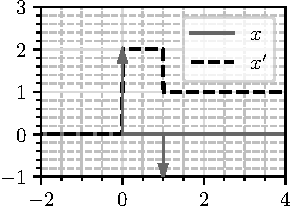
\includegraphics[scale=1]{fig/crtaj_ct_a.pdf}
        \caption{}
    \end{subfigure}
    \hspace*{0pt}\hfill
    \begin{subfigure}[c]{0.45\textwidth}
        \centering
        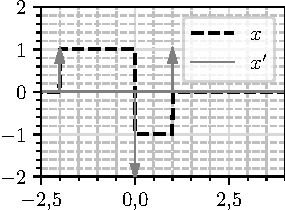
\includegraphics[scale=1]{fig/crtaj_ct_b.pdf}
        \caption{}
    \end{subfigure}
    \hfill
    \hspace*{0pt}

    \hspace*{0pt}\hfill
    \begin{subfigure}[c]{0.45\textwidth}
        \centering
        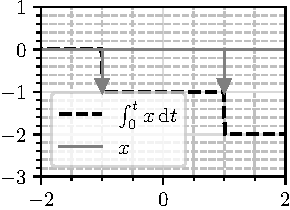
\includegraphics[scale=1]{fig/crtaj_ct_v.pdf}
        \caption{}
    \end{subfigure}
    \hspace*{0pt}\hfill
    \begin{subfigure}[c]{0.45\textwidth}
        \centering
        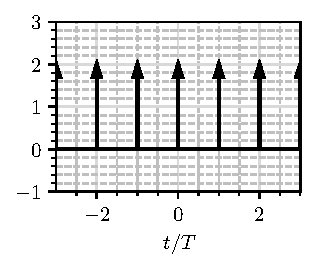
\includegraphics[scale=1]{fig/crtaj_ct_g.pdf}
        \caption{}
    \end{subfigure}
    \hfill
    \hspace*{0pt}

    \caption{}
\end{figure}
\vspace*{\ProblemSep}

\refstepcounter{ID}
\setcounter{fid}{0}
\graphicspath{{./1_uvod/1_osnovne_osobine_signala/}}
\noindent
\noindent
\textbf{\ID.}
Нацртати следеће
дискретне сигнале $x=x[n]$:
\begin{multicols}{2}
\begin{enumerate}
\item[(а)] $x[n] = \uu[n] - 2\uu[n-4]$, \\ и 
$y[n] = \nabla x[n]$;
\item[(б)] $x[n] = n^2( \updelta[n+2] - 2\updelta[n-2] )$, \\ и 
$y[n] = \sum_{k = -\infty}^n \hspace*{-0.5em}
 x[k]$;
\item[(в)] $x[n] = (1-n)(\uu[n+2] - \uu[n-3])$
\item[(г)]  $x[n] = \cos\dfrac{\uppi n}{N}  
\left(
\sum_{k = -\infty}^{\infty} \updelta[n-kN]
\right)  \uu[n] $, за $N = 3$;
\end{enumerate}
\end{multicols}
\noindent
где су $\uu[t]$ и $\updelta[n]$ дискретни 
јединични низ
и дискретни јединични импулс редом, a $\nabla x[n] = x[n] - x[n-1]$ је диференца уназад,
\vspace*{5mm}

\textsc{\underline{Резултат}}: 
Тражени дијаграми приказани су 
на слици \ID.1. \\
\begin{figure}[ht!]
    \hspace*{0pt}\hfill
    \begin{subfigure}[c]{0.45\textwidth}
        \centering
        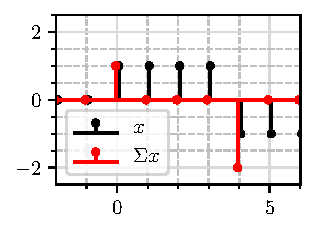
\includegraphics[scale=1]{fig/crtaj_dt_a.pdf}
        \caption{}
    \end{subfigure}
    \hspace*{0pt}\hfill
    \begin{subfigure}[c]{0.45\textwidth}
        \centering
        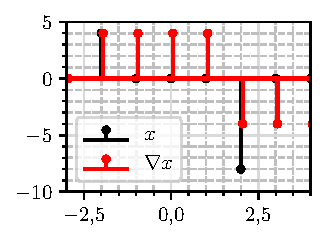
\includegraphics[scale=1]{fig/crtaj_dt_b.pdf}
        \caption{}
    \end{subfigure}
    \hfill
    \hspace*{0pt}

    \hspace*{0pt}\hfill
    \begin{subfigure}[c]{0.45\textwidth}
        \centering
        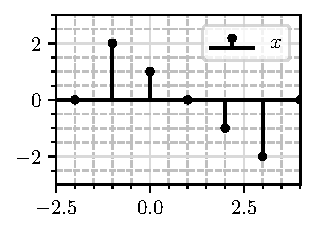
\includegraphics[scale=1]{fig/crtaj_dt_v.pdf}
        \caption{}
    \end{subfigure}
    \hspace*{0pt}\hfill
    \begin{subfigure}[c]{0.45\textwidth}
        \centering
        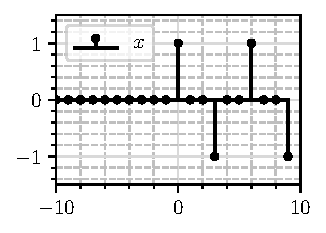
\includegraphics[scale=1]{fig/crtaj_dt_d.pdf}
        \caption{}
    \end{subfigure}
    \hfill
    \hspace*{0pt}
    \caption{Уз задатак \ID. На апсциси је $n$, а на ординати су означене величине.}
\end{figure}
\vspace*{\ProblemSep}

\refstepcounter{ID}
\setcounter{fid}{0}
\graphicspath{{./1_uvod/1_osnovne_osobine_signala/}}
\noindent
\textbf{\ID.} Изразити периодичну поворку Диракових импулса $\text{Ш}_T(t)$ 
сложеном трансформацијом 
јединичне периодичне поворке Диракових импулса $\text{Ш}(t) = \text{Ш}_1(t)$.

\indent 
\textsc{\underline{Решење}}: Период тражене поворке једнак је $T$ док је период јединичне поворке једнак
јединици. Јасно је потребно онда прво обавити скалирање временске осе тако да се од јединичног 
импулса добије импулс одговарајуће ширине. Том приликом је потребно обавити скалирање 
временске осе појединчаног Делта импулса\footnote{Користи се резултат 
$\updelta\bigl(a(t-t_0)\bigr) = \dfrac{1}{|a|} \updelta(t - t_0)$} па се има:
\begin{equation}
    \III\left(\dfrac tT\right) = 
    \sum_{k = -\infty}^{\infty} 
    \updelta \left( \dfrac tT - k \right)
    =
    \sum_{k = -\infty}^{\infty} 
    \updelta \left( \dfrac{t - kT}{T} \right) 
    = 
    \sum_{k = -\infty}^{\infty} 
    T \updelta \left( t - kT \right) 
    = T \III_T(t)
\end{equation}
Коначно, из добијеног резултата је тражени израз $\III_T(t) = \dfrac1T \III\left(\dfrac tT\right)$.
\vfill
\vspace*{\ProblemSep}

\refstepcounter{ID}
\setcounter{fid}{0}
\graphicspath{{./1_uvod/1_osnovne_osobine_signala/}}
\noindent
\subsubsection{\textit{Парност сигнала}}
\noindent
\PID \label{z:parnost}
Одредити парну и непарну компоненту 
континуалних сигнала $x =x(t)$ за:
\begin{multicols}{3}
\begin{enumerate}
\item[(а)] $x(t) = {\rm e}^{kt}$; и
\item[(б)] $x(t) = {\rm e}^{{\rm j}\upomega_0 t}$,
\end{enumerate}
\end{multicols}
\noindent
где су $k$ и $\upomega_0$ познате реалне константе. \\[2mm]

\textsc{\underline{Решење}}: 
Сваки континуални сигнал $x(t)$ може се, на \textit{јединствен} начин, представити преко његове парне и непарне компоненте, $x_{\rm e}(t) = {\rm Ev}\,x(t)$ и 
$x_{\rm o}(t) = {\rm Od}\,x(t)$ редом, као 
\begin{eqnarray}
    x(t) = x_{\rm e}(t) + x_{\rm o}(t).
    \label{eq:\ID.1}
\end{eqnarray}
Парна и непарна компонента сигнала могу се одредити
разматрањем израза за $x(-t)$ као и његове парне и непарне компоненте. Наиме,
\begin{equation}
    x(-t) = x_{\rm e}(-t) + x_{\rm o}(-t) \Rightarrow x(-t) = x_{\rm e}(t) - x_{\rm o}(t),
    \label{eq:\ID.2}
\end{equation}
при чему су искоришћени $x_{\rm e}(-t) = x_{\rm e}(t)$ и $x_{\rm o}(t) = -x_{\rm o}(-t)$, 
према дефиницији перне и непарне компоненте. Одатле се онда из система једначина 
\eqref{eq:\ID.1} и \eqref{eq:\ID.2} налазе изрази за парну и напарну компоненту сигнала датог као $x(t)$:
\begin{eqnarray}
    & x_{\rm e}(t) = \dfrac{ x(t) + x(-t) }{2},& \text{ и } \\
    & x_{\rm o}(t) = \dfrac{ x(t) - x(-t) }{2}.&
    \label{eq:\ID.3}
\end{eqnarray}


На основу добијеног резултата \eqref{eq:\ID.3}, онда се могу непосредно одредити парна и непарна компонента датих израза
\begin{enumerate}
    \item[(а)] ${\rm Ev} \{ {\rm e}^{kt} \} = \dfrac{ {\rm e}^{kt} + {\rm e}^{-kt} }{2} = \cosh(x)$, 
    и ${\rm Od}\{{\rm e}^{kt}\} =  \dfrac{ {\rm e}^{kt} - {\rm e}^{-kt} }{2} = \sinh(x)$;
    \item[(б)] ${\rm Ev}\{ {\rm e}^{{\rm j}\upomega_0 t}\} = \dfrac{ {\rm e}^{{\rm j}\upomega_0 t} + {\rm e}^{-{\rm j}\upomega_0 t} }{2} = \cos(\upomega_0 t)$,
    и ${\rm Od} \{ {\rm e}^{{\rm j}\upomega_0 t} \} =  \dfrac{ {\rm e}^{{\rm j}\upomega_0 t} - {\rm e}^{-{\rm j}\upomega_0 t} }{2} =\jj \sin(\upomega_0 t)$;
\end{enumerate}








\vspace*{\ProblemSep}

\refstepcounter{ID}
\setcounter{fid}{0}
\graphicspath{{./1_uvod/1_osnovne_osobine_signala/}}
\noindent
\noindent
\textbf{\ID}. 
Одредити парну и непарну компоненту 
континуалног простопериодичног сигнала, облика 
$x(t) = \sin \left(\upomega_0 t + \uptheta \right)$, где су $\upomega_0$ и $\uptheta$ позанте константе. 
\\[2mm]

\textsc{\underline{Решење}}: Решење се може потражити поступком описаним у задатку 
\ref{z:parnost}, ипак, у случају овог задатка, али и разних других сродних примера, резултат се може пронаћи 
\textit{идентификацијом} парног и непарног дела сигнала, трансформацијом полазног израза. Применимо израз за 
синус збира\footnote{Синус збира углова 
$\sin(\upalpha + \upbeta) = \sin\upalpha \cos\upbeta + \cos\upalpha \sin\upbeta$} чиме се добија 
\begin{equation}
    x(t) = \sin \left(\upomega_0 t + \uptheta \right) 
    = \underbrace{\cos \uptheta}_{\rm const} \cdot \sin \upomega_0 t + \underbrace{\sin \uptheta}_{\rm const} \cdot \cos \upomega_0 t.
\end{equation}
Пошто је познато да су $\sin(\upomega_0 t)$ и $\cos(\upomega_0 t)$ непаран и паран сигнал редом, а знамо да се 
сигнал $x(t)$ може на јединствен начин представити као збир његових парних и непарних компоненти, онда 
морају бити
\begin{eqnarray}
    {\rm Od} \{ x(t) \} = \cos \uptheta \cdot \sin \upomega_0 t,& \text{ и } \\
    {\rm Ev} \{ x(t) \}  = \sin \uptheta \cdot \cos \upomega_0 t.&
\end{eqnarray}

Овакав поступак идентификације компоненти сигнала, често може брже довести до резултата од поступка описаног у задаку 
\ref{z:parnost}.

\vspace*{\ProblemSep}

\refstepcounter{ID}
\setcounter{fid}{0}
\graphicspath{{./1_uvod/1_osnovne_osobine_signala/}}
\noindent
\noindent
\textbf{\ID}. 
Полазећи од дефиницијa парног и непарног сигнала
извести услов за парност сигнала
$$
	y(t) = x_1(t) \cdot x_2(t) \cdot x_3(t) \cdots x_n(t) = 
	\prod_{k = 1}^n x_k(t),
$$
где је сваки од сигнала $x_k(t)$ за $k \in \{1,2,\ldots,n\}$
или паран или непаран.
\\[2mm]

\textsc{\underline{Резултат}}: 
Сигнал је паран ако и само ако је број непарних сигнала из скупа $\{
x_1, x_2, \cdots, x_n\}$ паран. \\[5mm]


\vspace*{\ProblemSep}

\refstepcounter{ID}
\setcounter{fid}{0}
\graphicspath{{./1_uvod/1_osnovne_osobine_signala/}}
\noindent
\PID 
Применом својстава парних и непарних 
сигнала
израчунати вредности 
одређених интеграла 
\begin{multicols}{2}
\begin{enumerate}[label=(\alph*)]
\item
$\displaystyle 
I_1 = 
\int_{-\uppi/2}^{\uppi/2}
\dfrac{\cos t}{1 + {\rm e}^{\sin 2t}}
 \de t;
$

\item
$\displaystyle
I_2 = \int\limits_{-\uppi/3}^{\uppi/3}
\dfrac{1 - t + 2t^3 - t^5 + 2t^7}{\cos^2 (t)}\,{\rm d} t$.
\end{enumerate}
\end{multicols}

\textsc{\underline{Решење}}:
Пошто су границе интеграла парне, може се користити својство да је 
\begin{equation}
\displaystyle \int_{-a}^{a} f(t) \de t = 2\int_{0}^{a} {\rm Ev}\{f(t)\} \de t, \label{eq:\ID.1}
\end{equation}
односно, потребно је потражити парне компоненте датих подинтегралних величина. 

(а) Парна компоненте подинтегралне величине налази се применом особина парности простопериодичних функција, 
применом поступка из задатка \ref{z:parnost}, као 
\begin{eqnarray}
    {\rm Ev}\left\{  
        \dfrac{\cos t}{1 + {\rm e}^{\sin 2t}}
    \right\}
    &= \dfrac{
        \dfrac{\cos t}{1 + {\rm e}^{\sin 2t}} + \dfrac{\cos (-t)}{1 + {\rm e}^{\sin 2(-t)}}
    }{2}
    =
    \dfrac{
        \dfrac{\cos t}{1 + {\rm e}^{\sin 2t}} + \dfrac{\cos t}{1 + {\rm e}^{-\sin 2t}}
    }{2}
    =  \\
    &= \dfrac{ \dfrac{\cos(t) \cancel{( 2 + \ee^{\sin 2t} + \ee^{-\sin 2t} )} } { \cancel{2 + \ee^{\sin 2t} + \ee^{-\sin 2t}} } }{2}
    = \dfrac{1}{2} \cos(t).
\end{eqnarray}
Заменом добијеног резултата у \eqref{eq:\ID.1}, коначно се налази, $I_1 = 1$.

(б) Сличним поступком се налази резултат $I_2 = 2\sqrt 3$.

\vspace*{\ProblemSep}

\refstepcounter{ID}
\setcounter{fid}{0}
\graphicspath{{./1_uvod/1_osnovne_osobine_signala/}}
\noindent
\subsubsection{\textit{Периодичност, снага и енергија сигнала}}
\PID 
\noindent 
Утврдити да ли су следећи сигнали периодични и за оне који то јесу израчунати 
основни период:
\begin{multicols}{2}
\begin{enumerate}
\item[(а)] $x(t) = \cos(3t) + \sin(5t)$;
\item[(б)] $x(t) = \cos(6t) + \sin(\uppi t)$;
\item[(в)] $x(t) = \cos(6t) + \sin(8t) + {\rm e}^{{\rm j}2t}$.
\end{enumerate}
\end{multicols}

\textsc{\underline{Решење}}:
Периодичност збира континуалних сигнала $f_1(t)$, $f_2(t)$, $\ldots$, и $f_n(t)$ може се дискутовати на основу њихових основних 
периода $T_1$, $T_2$, $\ldots$, и $T_n$. Претпоставимо да је основни период сигнала 
$f(t) = f_1(t) + f_2(t) + \ldots + f_n(t)$ једнак $T$. Тада је јасно да се период сваког од сигнала сабирака 
мора садржати цео број пута у сигналу збира, односно $T = n_1T_1 = n_2T_2 = \ldots = n_nT_n$, где су $n_1$, $n_2$, $\ldots$, и $n_n$ 
цели бројеви. Пошто је основни период најмањи такав период, то значи да је $T$ најмањи број који се цео број пута 
садржи у сваком од периода сигнала сабирака, односно је
\begin{equation}
    T = {\rm NZS} \{ T_1, T_2, \ldots, T_n\}.
    \label{eq:nzs}
\end{equation}
Такав резултат ће постојати уколико је $\dfrac{T_i}{T_j} = \dfrac{n_i}{n_j} \in \mathbb Q, \forall i,j$,
односно, ако је однос сваког пара периода рационалан број.    
За такве периоде кажемо да су \textit{рационално самерљиви}.

\begin{enumerate}
    \item[(а)] Сигнал $x(t) = \cos(3t) + \sin(5t)$ је периодичан, јер су основни периоди\footnote{
    Основни период синусоиде $\sin(\upomega_0 t + \uptheta)$ је $T = 2\uppi /\upomega_0$.
    } сабирака рационално самерљиви, односно,  
    $T = {\rm NZS} \left\{ \dfrac{2\uppi}{3}, \dfrac{2\uppi}{5} \right\} = 2\uppi$. 
    \item[(б)] Сигнал $x(t) = \cos(6t) + \sin(\uppi t)$ је 
    апериодичан јер периоди сабирака, $\dfrac{2\uppi}{6}$ и $2$, нису рационално самерљиви пошто је 
    $\uppi \not\in \mathbb Q$.
    \item [(в)] Сигнал $x(t) = \cos(6t) + \sin(8t) + {\rm e}^{{\rm j}2t}$ је периодичан, 
    јер су основни периоди сабирака
    $\dfrac{\uppi}{3}$, $\dfrac{\uppi}{4}$, и $\uppi$ рационално самерљиви, а период
    је $T = {\rm NZS} \left\{ \dfrac{\uppi}{3}, \dfrac{\uppi}{4}, \uppi \right\} = \uppi$.
\end{enumerate}

\vspace*{\ProblemSep}
\subsection{Континуални системи
}

\refstepcounter{ID}
\setcounter{fid}{0}
\graphicspath{{./1_uvod/2_kontinualni_sistemi/}}
\noindent
\begin{slikaDesno}{fig/BG.pdf}[fig/BG-kolo.pdf]
\noindent
\textbf{{\color{red}*}\ID.}
На слици \ID.1 је приказана једна 
конструкција 
балистичког галванометра (БГ), 
инструмента за мерење протока 
наелектрисања. Казаљка инструмента
може да прави угаони отклон у границама
$0 \leq \upphi \leq \dfrac{\uppi}{2}$. Веза између струје, 
$i = i(t)$, на 
једином електричном приступу БГ
и угаоног отклона казаљке,
$\upphi = \upphi(t)$, 
дата је диференцијалном једначином
$
J \dfrac{\de^2 \upphi}{\de t^2}
+
F \dfrac{\de \upphi}{\de t}
+
K \upphi = \upalpha i,
\vspace*{1mm}
$ при чему је познато
$J = 6
\unit{s^2}$, 
$F = 24
\unit{s}
$, 
$K = 24$ и 
$\upalpha = \uppi{\rm e}
\unit{\dfrac{1}{\rm \upmu A}} \vspace*{1mm}$,
где је $\rm e$ основа природног логаритма.
Сматрати да се тај приступ
БГ, y електричном смислу, понаша као савршен кратак спој. Инструмент се калибрише на основу огледа са слике 2. 
Непосредно пре затварања прекидача, 
конданзатор је оптерећен количином наелектрисања 
$Q_0 = 1\unit{\upmu C}$
а казаљка БГ мирује у нултом положају,
$\upphi = 0$. (а)
Решавањем
у временском домену одредити 
кретање казаљке, 
$\upphi(t)$, по затварању прекидача до успостављања
новог стационарног стања.
(б) Скицирати 
временски дијаграм
$\upphi(t)$.
\end{slikaDesno}
(в) Израчунати 
вредности 
једнако размакнутих подеока са слике 1,
$Q_1$, $Q_2$, \ldots, $Q_6$,
ако се као показивање инструмента
(односно, количина 
наелектрисања протекла у импулсу) очитава вредност 
на коју показује казаљка у тренутку када је \myul{најдаље} од 
нултог подеока током свог кретања.\\

\textsc{\underline{Решење:}} На основу резултата задатка \ref{ID:capID}, струја која протиче кроз 
БГ по затваарању прекидача је $i(t) = Q_0 \updelta(t)$. Та импулсна побуда побуђује разматрани систем 
па је потребно потражити одзив на побуду. 

Карактеристични полином диференцијалне једначине система је 
$P(\uplambda) = J\uplambda^2 + F\uplambda + K$, корени карактеристичног полинома потражују се 
из обрасца решења квадратне једначине као 
$\uplambda_{1,2} = \dfrac{ -F \pm \sqrt{F^2 - 4JK} }{2J}$. Заменом бројних вредности установљава
се да постоји \textit{двоструки} реални корен $\uplambda_0 = -2\unit{s^{-1}}$. На основу тога, 
општи облик одзива на импулсну побуду се може записати у облику 
\begin{equation}
    \upphi(t) = (\Upphi_0 + \Upphi_1 t) \ee^{\uplambda_0 t}, \quad
    \text{где  су $\Upphi_0$ и $\Upphi_1$ произвољне константе}
    \label{eq:phi1}
\end{equation}
Користећи поступак за одређивање одзива на импулсну побуду из задатка 
\ref{ID:zadatakID}, закључујемо да одзив треба да има прекид у изводу првог реда, а да су 
остали изводи непрекидни. На основу тога је $\upphi(0^+) = 0$ и 
$\upphi'(0^+) = \dfrac{\upalpha Q_0}{J}$.

Из израза \eqref{eq:phi1} је $\upphi'(0^+) = \Upphi_0$ па је 
$\Upphi_0 = 0$. Имајући то у виду, први извод отклона казаљке у нули је 
$\upphi'(t) = \Upphi_1 \ee^{\uplambda_0 t}( \uplambda_0 t + 1 ) \Rightarrow 
\upphi'(0^+) = \Upphi_1
$, одакле се налази да је  
$\Upphi_1 = \dfrac{\upalpha Q_0}{J}$, па је 
$\Upphi_1 =  \dfrac{\uppi \ee}{6} \unit{s^{-1}}$. Коначно је тражени облик угаоног отклона казаљке 
дат изразом, $\upphi(t) = \dfrac{\upalpha Q_0}{J} t \ee^{\uplambda_0 t}$, односно бројевно 
$\upphi(t) = \dfrac{\uppi\ee}{6}\unit{s^{-1}} t 
\ee^{-2\unit{s^{-1}} t}$.  


(б) За цртање временског дијаграма најважнија је максималну тренутну вредност сигнала, будући
да се она користи у другом делиу задатка. 
нуле првог извода налазе се из ранијег резултата 
$\upphi'(t) = \Upphi_1 \ee^{\uplambda_0 t_{\rm m}} (\uplambda_0 t_{\rm m} + 1) = 0$ 
одакле је $t_{\rm m} = -\dfrac{1}{\uplambda_0} = \dfrac{1}{2}\unit{s}$ а максимална 
вредност је $\upphi_{\rm m} = \dfrac{\uppi}{12}\unit{rad}$. Додатно, могуће је одредити 
и тачку превоја за прецизније цртање, решавањем $\upphi''(t) = 0$ добија се да је тренутак превоја
$t_{\uppi} = 1\unit{s}$. Временски дијаграм тог резултата приказан је на слици 
\ref{fig:\ID.3}.

\begin{figure}[ht!]
    \centering
    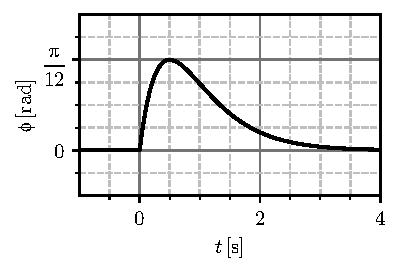
\includegraphics[scale = 1]{fig/BG_plot.pdf}
    \caption{}
    \label{fig:\ID.3}
\end{figure}

(в) Пошто је дати систем линеаран (описан је линеарном диференцијалном једначином), 
важи да уколико је побуда $1\unit{\upmu C} \updelta(t)$ произвела одзив 
$\upphi(t)$, онда ће побуда облика $k \unit{\upmu C} \updelta(t)$ произвести одзив
облика $k \upphi(t)$. Пошто је $\max k\upphi(t) = k \max \upphi(t) = \dfrac{k\uppi}{12}$,
а подеоци размакнути за по тачно $\dfrac{\uppi}{12}$, то подеоци треба да буду 
${Q_k = k\unit{\upmu C}}$.

\vfill

\vspace*{\ProblemSep}

\refstepcounter{ID}
\setcounter{fid}{0}
\graphicspath{{./1_uvod/2_kontinualni_sistemi/}}
\noindent
\textbf{\ID.}
Нека је систем описан диференцијалном једначином у облику
$\DS
P({\rm D})\,y(t) = x(t)$, где су $x(t)$ и $y(t)$ побуда и одзив тог система редом, а 
$P({\rm D})$ је оператор дат полиномом са реалним коефицијентима по оператору диференцирања 
${\rm D} = \dfrac{\de }{\de t}$. Полазећи од формуле одзива за експоненцијалну побуду, 
облика $y_{\rm p} = \dfrac{ \ee^{at} }{P(a)}$
, одредити 
партикуларни део одзива на нерезонантну побуду када је она простопериодична, облика 
(а) $x(t) = \cos(\upomega_0 t)$ и 
(б) $x(t) = \sin(\upomega_0 t)$.

\underline{\sc Решење:} Приметимо да је 
$\ee^{\jj\upomega_0 t} = \cos(\upomega_0 t) + \jj \sin(\upomega_0 t)$. Одзив на ту 

Мотивисани том примедбом, 
размотримо побуду комплексним сигналом облика: 
$\underline{x}(t) = x_{\rm r}(t) + \jj x_{\rm i}(t)$ 
\vspace*{\ProblemSep}

\refstepcounter{ID}
\setcounter{fid}{0}
\graphicspath{{./1_uvod/2_kontinualni_sistemi/}}
\noindent
\begin{slikaDesno}{fig/vrste_rl_0.pdf}
\PID
У колу са слике познато је 
$L = 1\unit{mH}$ и $R = 50\unit{\Upomega}$.
У почетном тренутку струја калема је 
$i_{L}(0^-) = 0,5\unit{mA}$. Напон побудног
генератора је облика 
$v_{\rm g}(t) = V_{\rm m} \sin(\upomega t)
\,{\rm u}(t)$, где су
$V_{\rm m} = 1\unit{V}$ и 
$\upomega = 10^6
\unit{\dfrac{rad}{s}}$. 
Као одзив се посматра 
струја калема на отпорнику $i_L = i_L(t)$.
%
Одредити (а) одзив на 
почетне услове, (б) одзив на побуду, 
(в) комплетан одзив и  
(г) устаљени одзив. 
\end{slikaDesno}

\textsc{\underline{Решење}}:
Диференцијална једначина која описује систем је 
\begin{equation}
    L \dfrac{{\de }i_L}{{\de t}} + R i_L = v_{\rm g}.
    \label{difeq}
\end{equation}
Њој одговара карактеристични полином $P(\uplambda) = R + L\uplambda$ који има само један реалан корен 
$\uplambda_0 = -\dfrac{R}{L} = - 5\times 10^4\,{\rm s}^{-1}$. Хомогени део решења ове диференцијалне 
једначине је стога $i_{L,\rm h}(t) = I_0 {\rm e}^{\uplambda_0 t}$, где је $I_0$ произвољна константа.
Партикуларни део се може одредити помоћу поступка показаног за нерезонантну синусоидалну побуду у задатку
\ref{ID:exp_sin_cos_pobude}, према 
\begin{equation}
i_{L, \rm p} = \mathbb I{\rm m}\left\{\dfrac{V_{\rm m}{\rm e}^{{\rm j}\upomega t}}{P({\rm j}\upomega)}
\right\} = 
\mathbb I{\rm m}\left\{
\dfrac{V_{\rm m}{\rm e}^{{\rm j}\upomega t}}{R + {\rm j}\upomega L}
\right\} = V_{\rm m}
\dfrac{ 
R \sin (\upomega t) - 
\upomega L \cos(\upomega t)
}{R^2 + (\upomega L)^2}. 
\end{equation}
Коначно, опште решење за струју калема је
\begin{equation}
i_{L}(t) = 
\underbrace{
I_0 {\rm e}^{\uplambda_0 t} }
_{\text{Хомогени део}}
+ 
\underbrace{
V_{\rm m}
\dfrac{ 
R \sin (\upomega t) - 
\upomega L \cos(\upomega t)
}{R^2 + (\upomega L)^2}}
_{\text{Партикуларни део}}
. 
\end{equation}

\vspace*{1mm}
(а) Одзив на почетне услове налази се само на
основу хомогеног дела, помоћу  
почетних услова. Добија се 
$$i_{L1}(t) = I_{01}{\rm e}^{\uplambda_0 t}
\Rightarrow
 i_{L1}(0^{-}) = 
 I_{01}\cancelto{1}{ {\rm e}^{\uplambda_0 \cdot 0} } \Rightarrow
 I_{01} = 0,5\unit{mA} .
$$
Тако да је одзив на почетне услве 
$i_{L1}(t) = 0,5\unit{mA}\,{\rm e}^{\uplambda_0 t}$. \\


(б) Одзив на побуду, одређује се заменом постиницијалних почетних услова у опште
решење диференцијалне једначине. Приликом тражења одзива на побуду претпоставља се да су сви 
преиницијални услови равни нули. Додатно, уколико у десној страни нема Диракових импулса 
онда су све функције $i_L(t), i_L'(t), i_L''(t), \dots, i_L^{(n-1)}(t)$ 
непрекидне, 
па су стога и постиницијални услови равни нули. У том облику тражи се \textit{другачија} 
константа за хомогени део.
\begin{equation}
\begin{aligned}
\underbrace{i_{L2}(0^+) = 0}
_{\text{Постиницијални услов}} = 
\underbrace{
I_{02} {\rm e}^{\uplambda_0 \cdot 0} }
_{\text{Хомогени део}}
+ 
\underbrace{
V_{\rm m}
\dfrac{ 
R \sin (\upomega \cdot 0) - 
\upomega L \cos(\upomega \cdot 0)
}{R^2 + (\upomega L)^2}
}
_{\text{Партикуларни део}}
& = 
I_{02} + \dfrac{\upomega L V_{\rm m} }{
R^2 + (\upomega L)^2} 
\Rightarrow \\
& = I_{02} \approx 1 \unit{mA}.
\end{aligned}
\end{equation}
Тако да је одзив побуду:
$
i_{L2}(t)
\approx 
1\unit{mA}\, {\rm e}^{\uplambda_0 t} 
+ 
50 \unit{\upmu A}\, \sin(\upomega t) -
1\unit{mA}\,
\cos (\upomega t).
$

(в) На основу суперпозиције, комплетан одзив добија се сабирањем одзива на почетне услове и 
одзива на побуду. Коначан резултат је валидан од тренутка $t=0$ услед чега 
се дописује одскочна функција. Коначно је комплетан одзив:
\begin{equation}
i_L(t) \approx
\bigl(1,5\unit{mA}\,{\rm e}^{\uplambda_0 t}
+
50 \unit{\upmu A}\, \sin(\upomega t) -
1\unit{mA}\,
\cos (\upomega t)
\bigr)
\,\uu(t).
\end{equation}
Приметимо да у овом изразу постоји члан 
добијен из хомогеног дела који је 
побуђен напонским генератором.  \\

(г) Након довољно дугог времена, чланови хомогеног дела који представљају прелазни
режим ишчезавају будући да је 
$e^{\uplambda_0 t} \to 0$ јер је 
$\uplambda_0 < 0$, након чега 
преостаје устаљени одзив
\begin{equation}
i_{L,\rm ss}(t) \approx 
50 \unit{\upmu A}\, \sin(\upomega t) -
1\unit{mA}\,
\cos (\upomega t).
\end{equation}

\vspace*{1mm}
\noindent
Добијени резултати су нацртани на 
дијаграмима на слици \ref{fig:\ID.2}.

\begin{figure}[ht!]
    \hspace*{0pt}\hfill
    \begin{subfigure}[t]{0.45\textwidth}
        \centering
        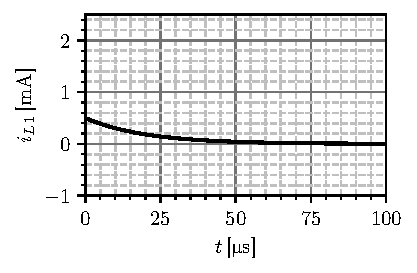
\includegraphics[scale=1]{fig/vrste_rl_1.pdf}
        \caption{Сопствени одзив.}
    \end{subfigure}
    \hspace*{0pt}\hfill
    \begin{subfigure}[t]{0.45\textwidth}
        \centering
        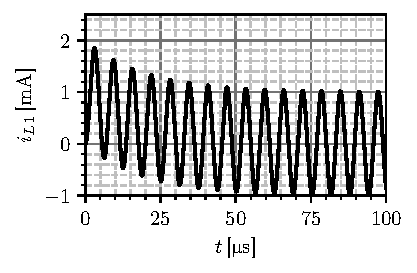
\includegraphics[scale=1]{fig/vrste_rl_2.pdf}
        \caption{Одзив на побуду.}
    \end{subfigure}
    \hfill
    \hspace*{0pt}

    \hspace*{0pt}\hfill
    \begin{subfigure}[t]{0.45\textwidth}
        \centering
        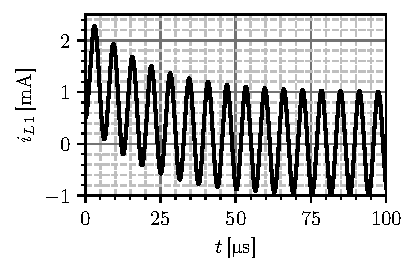
\includegraphics[scale=1]{fig/vrste_rl_3.pdf}
        \caption{Комплетан одзив}
    \end{subfigure}
    \hfill
    \hspace*{0pt}

    \caption{}
    \label{fig:\ID.2}
\end{figure}



\vspace*{\ProblemSep}

\refstepcounter{ID}
\setcounter{fid}{0}
\graphicspath{{./1_uvod/2_kontinualni_sistemi/}}
\noindent
\PID Нека је дат континуалан систем диференцијалном једначином облиика 
${y'(t) - ay(t)  = x(t)}$, где су $x(t)$ и $y(t)$ побуда и одзив тога система редом, а $a$ је позната
реална константа. Одредити одзив на експоненцијалну побуду облика 
${\rm e}^{bt} \, \uu(t)$, (а) ако је $b \neq a$ и (б) $b = a$. \\[5mm]

\textsc{\underline{Решење}}: За $t < 0$ је одзив на побуду једнак нули, док се 
за $t > 0$ решава диференцијална једначина 
${y'(t) - ay(t)  = {\rm e}^{bt}}$. У општем случају, решење се састоји из 
\textit{хомогеног} и \textit{партикуларног} дела. Хомогени део се налази одређивањем корена 
карактеристичног полинома $P(\uplambda) = \uplambda - a$ па је $\lambda_0 = a$. Постоји само 
једна карактеристична функција па је облик хомогеног дела одзива 
$y_{\rm h}(t) = A \ee^{at}$, за произвољну вредност константе $A$. Партикуларни део експоненцијалне побуде се тражи у 
експоненцијалном облику\footnote{То је природно за очекивати, будући да је експоненцијална функција
једина једнака своме изводу.}, па је $y_{\rm p} = B\ee^{bt}$, заменом у полазну једначину добија се:
\begin{equation}
    Bb\cancel{\ee^{bt}} - aB\cancel{\ee^{bt}} = \cancel{\ee^{bt}} \Rightarrow
    B = \dfrac{1}{b - a}.
\end{equation}
Комплетан облик одзива је онда облика $y(t) = A\ee^{at} + \dfrac{1}{b-a} \ee^{bt}$. Будући да је
побуда ограничена то је одзив непрекидан па је $y(0^+) = 0$ одакле се налази константа $A$, 
па је $A = \dfrac{1}{a - b}$, коначно се добија да је одзив на тражену побуду:
\begin{equation}
    y(t) = \dfrac{\ee^{bt} - \ee^{at}}{b - a}.
    \label{eq:\ID.1}
\end{equation}

(б) 
Проблем дељења нулом када је $b=a$ се може решити тражењем граничне вредности. 
Узмимо да је $b = a + \upepsilon$ 
и заменимо у резултат \ref{eq:\ID.1}, одатле се сређивањем даље има
\begin{equation}
    y(t) = \dfrac{\ee^{(a + \upepsilon)t} - \ee^{at}}{\cancel{a} + \upepsilon - \cancel{a}} = 
    \ee^{at} \dfrac{1 -\ee^{\upepsilon t}}{\upepsilon}.
\end{equation}
Будући да је $\DS \lim_{\upepsilon\to 0} \dfrac{1 -\ee^{\upepsilon t}}{\upepsilon} = t$ одзив
у траженом случају ће бити коначно 
$\DS y(t) = t \ee^{at}$.
\vspace*{\ProblemSep}

\refstepcounter{ID}
\setcounter{fid}{0}
\graphicspath{{./1_uvod/2_kontinualni_sistemi/}}
\noindent
\begin{slikaDesno}{fig/LC.pdf}
{\color{red}*}\PID  У колу са слике познати су 
$L = 100\unit{\upmu H}$ и $C = 1\unit{\upmu F}$.
У почетном тренутку у колу нема 
акумулисане енергије. Посматра
се систем чији је улаз напон побудног генератора $v_{\rm U} = v_{\rm U}(t)$ а излаз напон у колу 
$v_{\rm I} = v_{\rm I}(t)$. 
Познато је $v_{\rm I}(t < 0) = 0$ а побуда
је у облику $v_{\rm U}(t) = V_{\rm m} 
\sin(\upomega t)\,{\rm u}(t)$, где је 
$V_{\rm m} = 10\unit{mV}$. Одредити 
и скицирати напон на 
излазу система када је кружна учестаност 
побудног генератора (а) $\upomega = 10^3 
\unit{\dfrac{rad}{s}}$ и (б) 
$\upomega = 10^5 
\unit{\dfrac{rad}{s}}$. За учестаност из 
тачке (б) скицирати и (в) дијаграм снаге 
коју улаже напонски генератор у колу
$p_{\rm g} =p_{\rm g}(t)$.
\end{slikaDesno}\\

\textsc{\underline{Резултат}}:

(а) Тражени одзив је $v_{\rm I}(t) = 10\unit{mV} \sin(\upomega t)$. 
Резултат је приказан на слици \ref{fig:\ID.a}.\\[2mm]

(б) Тражени одзив је $v_{\rm I}(t) = -0,5\unit{\dfrac{V}{ms}} t \cos(\upomega t)$.
Резултат је приказан на слици \ref{fig:\ID.b}.\\[2mm]

(в) Тражена снага је $p_{\rm g} \approx 250\unit{\dfrac{\upmu W}{ms}} t
\bigl(1 + \cos(2\upomega t) \bigr)$.
Резултат је приказан на слици \ref{fig:\ID.v}. \\

\noindent
\begin{figure}[ht!]
    \hspace*{0pt}%\hfill
    \begin{subfigure}[b]{0.32\textwidth}
        %\centering
        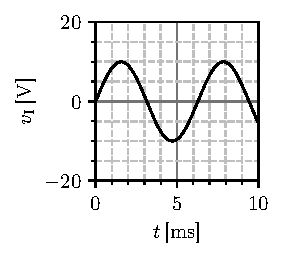
\includegraphics[scale=1]{fig/LC_a.pdf}
        \caption{}
        \label{fig:\ID.a}
    \end{subfigure}
    %\hfill
    \begin{subfigure}[b]{0.32\textwidth}
        %\centering
        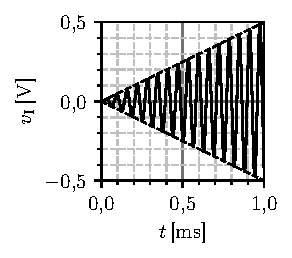
\includegraphics[scale=1]{fig/LC_b.pdf}
        \caption{}
        \label{fig:\ID.b}
    \end{subfigure}
    %\hfill
    \begin{subfigure}[b]{0.32\textwidth}
        %\centering
        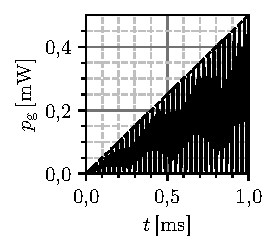
\includegraphics[scale=1]{fig/LC_v.pdf}
        \caption{}
        \label{fig:\ID.v}
    \end{subfigure}
    %\hfill
    %\hspace*{0pt}
    \caption{}
    \label{fig:\ID.2}
\end{figure}




\vspace*{\ProblemSep}
\section{Фуријеови редови континуалних и дискретних сигнала}
\subsection{Фуријеови редови континуалног сигнала}

\refstepcounter{ID}
\setcounter{fid}{0}
\graphicspath{{./2_furijeovi_redovi/1_kontinualni/}}
\noindent
\begin{slikaDesno}{fig/rect-per15.pdf}
    \textbf{\ID.}\label{ID:rect_pulse_train_FS} 
    Дат jе напонски сигнал $v = v(t)$ облика периодичне поворке униполарних правоугаоних 
    импулса амплитуде ${V_{\rm m} = 5\unit{V}}$, као на слици. Трајање импулса је $DT$ где је 
$D = 25\%$ (тзв. \textit{фактор испуне}), а учестаност jе $f = 1\unit{kHz}$. 
Одредити развоj овог сигнала у комплексан Фуриjеов ред, $V[k]$, на основном периоду $T$.
\end{slikaDesno} \\

\textsc{\underline{Решење}}: Развој у Фуријеов ред се може потражити по дефиницији применом 
аналитичке релације 
$\DS V[k] = \int_{\langle T \rangle} v(t) \ee^{-\jj k \upomega_{\rm F} t} \, \de t$, 
поступком\footnote{Користи се резултат $\int e^{kx} \, \de x = \frac{1}{k} e^x + C$}
\begin{align}
    V[k] = \int_{0}^T v(t) \ee^{-\jj k \upomega_{\rm 0} t} \, \de t 
         = \int_{0}^{DT}  V_{\rm m} \ee^{-\jj k \frac{2\uppi}{T} t} \, \de t
         = -\dfrac{V_{\rm m}}{\jj k \frac{2\uppi}{T}} 
         \ee^{-\jj k \frac{2\uppi}{T} t}\bigg|_{t = 0}^{t = DT}
         = V_{\rm m}\dfrac{
            1
            -
            \ee^{-\jj k 2\uppi D}
         }{\jj k \frac{2\uppi}{T}} 
\end{align}
Добијени облик може се поједноставити примедбом 
$\sin(x) = \dfrac{\ee^{\jj x} - \ee^{-\jj x}}{\jj 2} = \ee^{\jj x} \dfrac{1 - \ee^{-\jj 2x}}{\jj 2}$,
односно, 
$\dfrac{1 - \ee^{-\jj 2x}}{\jj 2} = \ee^{-\jj x} \sin(x) $,
одакле се може писати
\begin{align}
    V[k] = V_{\rm m}DT 
     \underbrace{
     \dfrac{
        1
        -
        \ee^{-\jj 2 (k \uppi D) }
     }{\jj 2 }}_{ = \ee^{-\jj k \uppi D/2} \sin(k\uppi D) }
     \cdot 
     \dfrac{1}{k \uppi D} 
     = V_{\rm m} D T \dfrac{\sin(k\uppi D)}{k\uppi D} \ee^{-\jj k \uppi D/2} 
     = V_{\rm m} D T \sinc(k \uppi D) \ee^{-\jj k \uppi D/2}.
\end{align}
Добијени резултат може се одредити и таблично којом приликом ће се члан 
$\ee^{-\jj k \uppi D/2}$ појавити услед кашењења у времену периодичне поворке правоугаоних 
импулса симетричне око ординате. 

\vspace*{\ProblemSep}

\refstepcounter{ID}
\setcounter{fid}{0}
\graphicspath{{./2_furijeovi_redovi/1_kontinualni/}}
\noindent
\begin{slikaDesno}{fig/exp_osc.pdf}
\PID У колу са слике познато је 
$R = 1\unit{k\Upomega}$, $C=1\unit{\upmu F}$ и 
напон напајања $V_{\rm CC} = 5\unit{V}$.
Систем „К“ управља идеалним прекидачем П 
на основу напона $v_{C}$. Прекидач П је иначе 
отворен, уколико напон $v_{\rm C}$ достигне вредност 
$mV_{\rm CC}$, где је $0 \leq m \leq 1$ позната 
константа, контролни систем „K“ тренутно и 
\textit{краткотрајно} затвара прекидач. У почетном 
тренутку је $v_{\rm C}(0) = 0$. 
\begin{enumerate}[label=(\alph*)]
\item Одредити  напон 
на кондензатору у зависности од времена, и нацртати његов временски 
дијаграм за $m = \dfrac{1}{2}$; и
\item одредити спектралне коефицијенте 
тог напона на његовом основном периоду у устаљеном 
сложенопериодичном режиму. 
\end{enumerate}
\end{slikaDesno} \\


\underline{\sc Решење:} 

(а) Кондензатор се пуни струјом из извора напајања, напона $V_{\rm CC}$,  
преко отпорника отпорности $R$. Израз за напон кондензатора у том случају је 
\begin{equation}
v_{C}(t) = V_{\rm CC} \left(
    1 - \ee^{-t/\uptau} 
\right), \label{eq:\ID.vc}
\end{equation} где је $\uptau = RC$ временска константа посматраног система првог реда. Пуњење кондензатора траје
све док је $v_C(t) < m V_{\rm CC}$. У граничном случају је, 
$v_C(T) = m V_{\rm CC}$, одатле се може одредити тренутак $T$ када се први пут затвара прекидач. 
Има се резултат
\begin{equation}
    \cancel {V_{\rm CC}} \left(
    1 - \ee^{-T/\uptau} \right) = m \cancel{V_{\rm CC}}
    \Rightarrow \ln(1 - m) = -\dfrac{T}{\uptau} \Rightarrow 
    T = \uptau \ln \left( \dfrac{1}{1 - m} \right).
\end{equation}

Након затварања прекидача је $v_{C}(T^+) = 0$, односно, краткотрајно затварање идеалног прекидача 
у потпуности растерећује кондензатор, након чега се пређашњи процес понавља. 
Односно, процес описан изразом \eqref{eq:\ID.vc} у домену 
$\DS 0 < t < T = \uptau \ln \left( \dfrac{1}{1 - m} \right)$, представља основни период напона
на кондензатору. 

Уколико се замене дате вредности има се да је временска константа 
$\uptau = 1\unit{ms}$, и да је $T = \uptau \ln 2 \approx 0,69 \unit{ms}$. 
Тражени временски дијаграм приказан је на слици \ref{fig:\ID.2}. На истом дијаграму, испрекиданом
линијом приказан је и продужетак дијаграма првобитног пуњења кондензатора -- који илуструје да би 
у недостатку прекидача тај напон асимптотски растао до напона напајања. 

\begin{figure}[ht!]
    \centering
    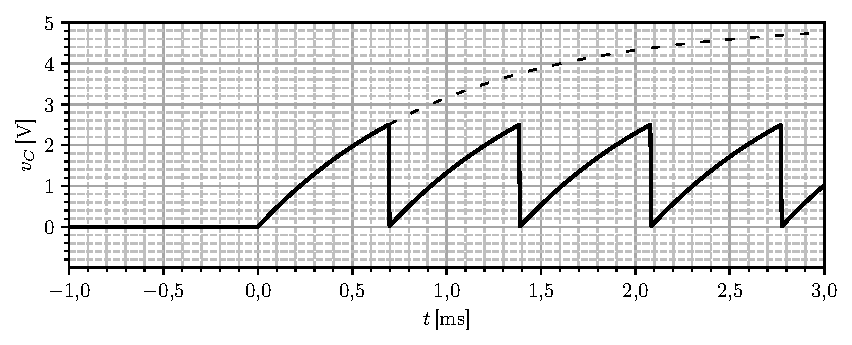
\includegraphics[scale=1]{fig/exp_osc_plot.pdf}
    \caption{Пример временског дијаграма за $m = \dfrac{1}{2}$, $V_{\rm CC} = 5\unit{V}$. }
    \label{fig:\ID.2}
\end{figure} 

(б) Развој у Фуријеов ред може се поједноставити применом особине суперпозиције
$\FS{ v_C(t) } = 
\FS{ V_{\rm CC} \left(
    1 - \ee^{-t/\uptau} \right) } 
= V_{\rm CC} \left(
    \FS{1}
    -
    \FS{
    \ee^{-t/\uptau}    
    }
\right) 
= V_{\rm CC} \left(
\updelta[k] 
-
\FS{
    \ee^{-t/\uptau}    
    }
\right).
$ 
Развој преосталог члана, експоненцијалног сигнала, у Фуријеов ред може се обавити по 
дефиницији\footnote{
    Развој у Фуријеов ред по дефиницији 
    $\DS\FS{x(t)} = \dfrac{1}{T}\int_{\langle T \rangle} x(t) \ee^{-\jj k \upomega_{\rm F} t} \de t$.
}, за $\upomega_{\rm F} = \upomega_0$
решавањем интеграла\footnote{Користи се интеграл 
    $\int e^{kx} \de x = e^{kx}/k + C$.
} 
\begin{equation}
    \FS{
    \ee^{-t/\uptau}    
    }
    = \dfrac{1}{T}\int_0^T 
    \ee^{-t/\uptau} \ee^{-\jj k \upomega_0 t} \,\de t
    =
    \dfrac{1}{T}\int_0^T 
    \ee^{-\left( \jj k\upomega_0  +  1/\uptau \right) t } \,\de t
    = 
    -\dfrac{
        \ee^{-\left( \jj k \cancelto{2\uppi}{\upomega_0 T}  +  T/\uptau \right) }
        - 1
    }{ \jj k \cancelto{ 2\uppi }{\upomega_0 T}  +  T/\uptau }.
\end{equation}
Приметимо да је 
$
\ee^{ -\left( \jj 2\uppi k  +  T/\uptau \right)} 
= \cancelto{1}{\ee^{\jj 2\uppi k}} + {1-m} = 2 - m$, па се коначно има: 
$
\FS{
    \ee^{-t/\uptau}    
    } =
    \dfrac{m - 1}{
        \jj 2\uppi k - \ln\left( 1 - m \right)
    }.
$ Коначно, добија се да је развој траженог сигнала у Фуријеов ред дат изразом
$V_C[k] = 
V_{\rm CC} \left(
    \updelta[k] 
        - 
        \dfrac{m - 1}{
            \jj 2\uppi k - \ln\left( 1 - m \right)
        }
\right)$. \\

Представљени систем представља једно принципско решење за пројектовање осцилатора 
(тзв. \textit{релаксациони осцилатор}). Променом границе укључења контролера који практично
ресетује напон кондензатора, односно променом 
параметра $m$,
мења се учестаност осциловања. Систем за контролу „К“ може се реализовати са једним операционим
појачавачем који се понаша као компаратор, док је прекидач могуће реализовати као нпр. MOS 
транзистор. 

\vspace*{\ProblemSep}

\refstepcounter{ID}
\setcounter{fid}{0}
\graphicspath{{./2_furijeovi_redovi/1_kontinualni/}}
\noindent
\newpage
\begin{slikaDesno}{fig/proc_1.pdf}[fig/proc_2.pdf]
    \noindent
    \textbf{{\color{red}*}\ID.}
    На слици \ID.1 jе представљена принципска шема система за
    генерисање и довођење сигнала такта до одговараjућег прикључка
    дигиталног процесора. Генератор такта jе идеалан напонски
    генератор симетричне униполарне поворке правоугаоних импулса
    учестаности
    $f_{\rm clk} = \dfrac{1}{T_{\rm clk}} = 4\unit{MHz}$
    и амплитуде $V_{\rm m} = 5\unit{V}$. 
    Линиjа за пренос такта моделуjе се као као каскадна
    веза идеалног блока за кашњење, кашњења 
    $\uptau = 125\unit{ns}$, и идеаланог филтра пропусника ниских учестаности,чиjа
    jе фреквенциjска преносна карактеристика 
    $H(\jj\upomega) = \rect\left( \dfrac{\upomega}{2\upomega_0} \right)$, где је 
    $\upomega_0$ непознати параметар. 
    Према спецификациjи употребљеног процесора, при
    преласку напона такта са ниског на високи ниво, дозвољено jе
    да у прелазноj зони између $V_1 = 1,5\unit{V}$ и $V_2 = 3,5\unit{V}$, доведени сигнал такта
    проведе наjвише 
    $\Delta t_{\rm max} = 5\unit{ns}$, као што jе илустровано на слици \ID.2. 
    \end{slikaDesno}

    (а) Одредити развоjе генерисаног сигнала такта, $v_{\rm clk}(t)$, и сигнала такта
    на улазу у процесор $v_{\rm clk}^{\rm(CPU)}(t)$ у комплексан Фуријеов ред у зависности 
    од параметра $\upomega_0$.
    (б) Одредити коефицијенте развоја сигнала $\dfrac{\de v_{\rm clk}^{\rm (CPU)}(t)}{\de t}$ 
    у комплексан Фуријеов ред.  
    (в) Одредити параметар $\upomega_0$ тако да буде задовољена наведена спецификација датог 
    процесора. 

    \underline{\it Напомена.} Приликом прорачуна времена које сигнал такта проводи у 
    прелазној зони, претпоставити да је нагиб сигнала такта 
    $\dfrac{\de v_{\rm clk}^{\rm (CPU)}(t)}{\de t}$ практично константан и да има максималну 
    вредност. \\

    \textsc{\underline{Решење}}: Генерисани сигнал такта јесте периодична поворка правоугаоних импулса. 
    Спектар такве поворке, на основном периоду $T_{\rm clk}$, на основу резултата задатка 
    \ref{ID:rect_pulse_train_FS} је $V_{\rm clk}[k] = 
    (-\jj)^k \dfrac{V_{\rm m}}{2} \sinc \left(
    \dfrac{k}{2}
    \right) $.
    Модел линије за пренос сачињен је из каскадне везе идеалног филтра и линије за 
    кашњење $T[k] = \rect \left( \dfrac{k{\upomega_{\rm clk}}}{2\upomega_0} \right) 
    \cdot \ee^{-\jj k {\upomega_{\rm clk}\uptau}} = 
    \rect \left( \dfrac{k{\upomega_{\rm clk}}}{2\upomega_0} \right) 
    \cdot (-1)^k$. Спектар напона на улазу у процесор онда је коначног облика 
    \begin{equation}
        V_{\rm clk}^{\rm (CPU)}[k] 
        = T[k] \cdot V_{\rm clk}[k] 
        =  
        \dfrac{\jj^{k} V_{\rm m}}{2}
        \rect \left( \dfrac{k{\upomega_{\rm clk}}}{2\upomega_0} \right) 
        \cdot
        \sinc \left(
        \dfrac{k}{2} \right)
    \end{equation}

    (б) Применом правила извода\footnote{Правило извода је 
    $
    \mathcal{FS}\left\{\dfrac{\de x(t)}{\de t}\right\} = \jj k \upomega_{\rm 0} 
    \mathcal{FS}\left\{ x(t) \right\} $ \\[1mm]} добија се резултат
    \begin{equation}
        \FS{ \dfrac{v_{\rm clk}^{\rm (CPU)}}{\de t}} [k]
        = 
        \dfrac{ 
        \jj^{k+1} \,
        k \upomega_{\rm clk} \, 
        V_{\rm m} }{2}
        \rect \left( \dfrac{k{\upomega_{\rm clk}}}{2\upomega_0} \right) 
        \cdot
        \sinc \left(
        \dfrac{k}{2} \right)
    \end{equation}

    (в) 
    Због симетрије, током преласка кроз средину прелазне зоне, сигнал има максималан нагиб у тренутку 
    $t = \uptau$, будући да је и ивица сигнала за толико закашњена. По претпоставци из напомене 
    са таквим нагибом нагибом треба да пређе целу прелазну зону за највише време 
    $\Delta t_{\rm max}$. Односно треба да важи
    \begin{equation}
        \dfrac{ v_{\rm clk}^{\rm (CPU)} }{\de t} (\uptau) > \dfrac{\Delta V}{\Delta t_{\rm max}}
        = 0,4\unit{\dfrac{V}{ns}}  \label{eq:\ID.uslov}
    \end{equation}

    Вредност извода у том тренутку потражује се на основу синтетичке релације\footnote{
    Користи се у облику $x(\uptau) = \sum_{k = -\infty}^{\infty} X[k] \ee^{\jj k\upomega_{\rm F} \uptau}$
    } Фуријеовог реда као 
    \begin{align}
        \dfrac{v_{\rm clk}^{\rm (CPU)}}{\de t}  (\uptau)
        =& 
        \sum_{k = \infty}^{\infty} 
        \FS{ \dfrac{v_{\rm clk}^{\rm (CPU)}}{\de t} }[k] \, \ee^{\jj k \upomega_{\rm clk} \uptau} 
        = 
        \FS{ \dfrac{v_{\rm clk}^{\rm (CPU)}}{\de t} }[k] \, (-1)^k \\[1.5mm]
        =&
        \sum_{k = \infty}^{\infty} 
        \dfrac{ 
        (-1)^k \jj^{k+1} k \upomega_{\rm clk} \, 
        V_{\rm m} }{2}
        \rect \left( \dfrac{k{\upomega_{\rm clk}}}{2\upomega_0} \right) 
        \cdot
        \sinc \left(
        \dfrac{k}{2} \right). \label{eq:\ID.dvtau}
    \end{align}
    За израчунавање суме распишимо да је 
    $k \sinc\dfrac{k}{2} = 
    \cancel{k} \dfrac{\sin\left( \frac{k\uppi}{2} \right) }{ \frac{\cancel{k}\uppi}{2} }
    $, те приметимо да је \linebreak
    ${\sin\left( \frac{k\uppi}{2} \right) = 
    \begin{cases}
        (-1)^m ,&  k = 2m+1 \\
        0      ,& k = 2m
    \end{cases}}$. Заменом добијених резултата  
    у $\eqref{eq:\ID.dvtau}$ и сређивањем помоћу 
    $ (-1)^k \jj^{k+1} \bigg|_{k = 2m+1} = 
    (-1)^{2m + 1} \jj^{2m + 2} = (-1)^m
    $
    ,има се 
    $
        \dfrac{v_{\rm clk}^{\rm (CPU)}}{\de t}  (\uptau)
        = \DS
        \sum_{\substack{ k = -\infty \\ k = 2m + 1 } }^{\infty} 
        \dfrac{ 
        \upomega_{\rm clk} \, 
        V_{\rm m} }{\uppi}
        \rect \left( \dfrac{{k \upomega_{\rm clk}}}{2\upomega_0} \right)  
    $. Вечичина под сумом је парна функција па се може одговарајућа\footnote{
        Трансформација за парни сигнал $a[k]$ је 
        $\sum_{k = -\infty}^{\infty} a[k] = a[0] + 2\sum_{k = 1}^{\infty} a[k]$.
    }
    трансформација. Добијена сума се онда може
    може средити изражавањем правоугаоног импулса у облику
    $
        \rect \left( \dfrac{{k \upomega_{\rm clk}}}{2\upomega_0} \right)
        =
        \begin{cases}
            1,& k < \dfrac{\upomega_{\rm 0}}{\upomega_{\rm clk}} \\[5mm]
            0,& k > \dfrac{\upomega_{\rm 0}}{\upomega_{\rm clk}} 
        \end{cases}
    $, што се може искористити за постављање горње границе коначне суме:
    $
        \dfrac{v_{\rm clk}^{\rm (CPU)}}{\de t}  (\uptau)
        = \DS
        \sum_{\substack{ k = -\infty \\ k = 2m + 1 } }^{k < \upomega_0 / \upomega_{\rm clk} } 
        \dfrac{ 2
        \upomega_{\rm clk} \, 
        V_{\rm m} }{\uppi} 
    $. Број чланова добијене суме јесте $М$, број непарних бројева између $0$ и 
    $\dfrac{\upomega_0}{\upomega_{\rm clk}}$, а који има смисао   
    броја непарних хармоника сигнала такта које пропушта филтар.  
    \\[2mm]
    
    
    Одавде се има 
    $\dfrac{\de v_{\rm clk}^{\rm (CPU)}}{\de t} (\uptau)
    = 
    M
    \dfrac{ 2
        \upomega_{\rm clk} \, 
        V_{\rm m} }{\uppi} 
    $, на основу услова из \eqref{eq:\ID.uslov}, заменом бројевних вредности налази се услов 
    за број непарних хармоника које филтар треба да пропусти. Одавде се има услов да је 
    $M = 
    \dfrac{\uppi} { 2
        \upomega_{\rm clk} \, 
        V_{\rm m} } 
    \dfrac{\de v_{\rm clk}^{\rm (CPU)}}{\de t} (\uptau)
    > 12,5 \unit{\dfrac{ns}{V}} \cdot 0,4 \unit{\dfrac{nV}{s}} = 5$. Односно, филтар мора да пропусти
    \textit{барем} 5 \textit{непарних} хармоника побудног сигнала, а то су
    $\upomega_{\rm clk}$, $3\upomega_{\rm clk}$, $5\upomega_{\rm clk}$, $7\upomega_{\rm clk}$, и
    $9\upomega_{\rm clk}$, односно, мора бити да је 
    $\upomega_0 > 9\upomega_{\rm clk}$, или 
    $f_0 > 9f_{\rm clk} = 36\unit{MHz}$.    
 
    У овом задатку је илустровано, да је стримина ивице правоугаоних импулса сразмерна
    броју хармоника које пропушта филтар. На слици \ID.3 илустрован је резултат. 
    Црвеним областима обележени су габарити унутар којих сигнал не сме да пролази, 
    односно назначене су границе прелазне зоне по времену и по напону. Нацртани су сигнали 
    са 1--5 непарних хармоника, и на слици може да се види да су са најмање 5
    непарних хармоника задовољени
    тражени габарити. 

    \begin{figure}[ht!]
        \centering
        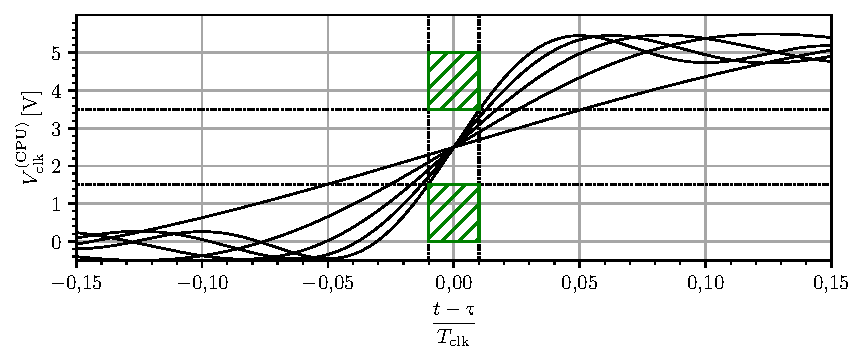
\includegraphics[scale=1]{fig/proc_plot.pdf} 
        \caption{}
    \end{figure}
\vspace*{\ProblemSep}
\section{Фуријеова трансформација континуалних и дискретних сигнала}
\subsection{Фуријеова трансформација континуалног сигнала}

\refstepcounter{ID}
\setcounter{fid}{0}
\graphicspath{{./3_furijeove_tranformacije/1_CT/}}
\noindent
\begin{slikaDesno}{fig/rect_pulse_0_T.pdf}
\PID 
\label{ID:rect_pulse_spectrum}
На слици \ID.1 приказан је правоугаони импулс јединичне амплитуде 
ширине $T$, са почетком у нули. Одредити Фуријеову трансформацију тог сигнала. \\

\hspace{4mm}
\textsc{\underline{Решење}:} Дати сгинал се може записати у облику 
$x(t) = \uu(t) - \uu(t - T)$. Применом особине померања у времену Фуријеове трансформације\footnotemark
и табличног резултата $\mathcal{FT}\{\uu(t)\} = \dfrac{1}{\jj\upomega} + \uppi\updelta(\upomega)$,
има се резултат
$X(\jj\upomega) = \dfrac{1}{\jj\upomega} + \uppi \updelta(\upomega) - 
        \dfrac{\ee^{-\jj\upomega T}}{\jj\upomega} - \uppi \ee^{-\jj\upomega T}\updelta(\upomega) 
        =\dfrac{1 - \ee^{-\jj\upomega T} }{\jj\upomega} + 
        \cancelto{0}{
        \uppi(\underbrace{1 - \ee^{-\jj\upomega T}}_{=0 \text{ за } \upomega = 0}) \updelta(\upomega)
        }$, где је у последњем кораку примењено својство еквиваленције Дираковог импулса. 
Коначно је $X(\jj\upomega) = \dfrac{1 - \ee^{-\jj\upomega T} }{\jj\upomega}$
\end{slikaDesno}
\footnotetext{Својство померања ФТ је $\mathcal{FT}\{x(t-T)\} = \mathcal{FT}\{x(t)\}\cdot\ee^{-\jj\upomega T}$.}



\vspace*{\ProblemSep}
\subsection{Фуријеова трансформација дискретног сигнала}
\section{Лапласова трансформација}
\subsection{Системи диференцијалних једначина}

\refstepcounter{ID}
\setcounter{fid}{0}
\graphicspath{{./4_laplasova_transformacija/2_sistemi_dif_jna/}}
\noindent
\begin{slikaDesno}{fig/LC_izbijanje.pdf}
    \textbf{{\color{red}*}\ID.} 
    У колу са слике познати су 
    $L$, 
    $C$ и коефицијент магнетске спреге $k \ll 1$.
    У почетном тренутку су познати 
    $i_2(0) = v_1(0) = v_2(0) = 0$ и 
    $i_1(0) = I_0$. Поставити (а)
    систем 
    интегро-диференцијалних једначина кола 
    по струјама $i_1$ и $i_2$. Помоћу 
    Лапласове
    трансформације (б) одредити струју $i_1(t)$.
    Скицирати (в) временски дијаграм 
    добијеног одзива
    $i_1(t)$ за $t > 0$.
\end{slikaDesno} \\

\textsc{\underline{Решење}}:
Напоне $v_1$ и $v_2$ са једне стране повезују струјно-напонске карактеристике
спрегнутих калемова дата је системом једначина 
\begin{eqnarray}
    v_1 = L_1 \dfrac{\de i_1}{\de t} + L_{12} \dfrac{\de i_2}{\de t} \\
    v_2 = L_{21} \dfrac{\de i_1}{\de t} + L_{2} \dfrac{\de i_2}{\de t},
\end{eqnarray}
При чему су, по услову задатка, $L_1 = L_2 = L$ и $L_{12} = L_{21} = kL$. Са друге стране, 
напон и струја су повезани према карактеристици кондензатора\footnote{
Полазећи од израза за струја што се може записати у интегралној форми као 
$\DS v_{\rm 1} = - \dfrac{1}{C} \int_{0}^{t} i_1 \de \uptau$, односно
$\DS v_{\rm 2} = - \dfrac{1}{C} \int_{0}^{t} i_2 \de \uptau$.
Заменом у израз за струју кондензатора $i_{\rm C} = C \dfrac{\de v_C}{\de t}$, интеграљењем
обе стране се добија коришћена напонско-струјна карактеристика.
} при неусклађеним референтним 
смеровима резултата, у систем једначина спрегнутих калемова и даљим сређивањем добија се 
\begin{eqnarray}
    - \dfrac{1}{C} \int_{0}^{t} i_1 \de \uptau = L \dfrac{\de i_1}{\de t} + kL \dfrac{\de i_2}{\de t}; 
    & \Rightarrow & 
    \dfrac{\de i_1}{\de t} + k \dfrac{\de i_2}{\de t} + \upomega_0^2 \int_0^t i_1 \, \de \uptau = 0
    \\
    - \dfrac{1}{C} \int_{0}^{t} i_2 \de \uptau = kL \dfrac{\de i_1}{\de t} + L \dfrac{\de i_2}{\de t}
    & \Rightarrow &
    k \dfrac{\de i_1}{\de t} + \dfrac{\de i_2}{\de t} + \upomega_0^2 \int_0^t i_2 \, \de \uptau = 0,
\end{eqnarray}
где је $\upomega_0 = \dfrac{1}{\sqrt{LC}}$. Добијени систем интегро-диференцијалних једначина 
описује понашање посматраног система \\

(б) Добијени систем једначина преводи се у фреквенцијски домен применом правила диференцирања 
уз почетни услов\ и правила интеграљења\footnote{Правило диференцирања $\mathcal{L} \left\{ \dfrac{\de x(t)}{\de t} \right\}
= s X(s) - x(0^+)$; Правило интеграљења 
$\DS \mathcal{L} \left\{ \int_{0^-}^{t} f(\uptau) \, \de \uptau \right\} = \dfrac{1}{s} F(s)$. }. 
Нека су $I_1 = I_1(s)$ и $I_2 = I_2(s)$, онда је
\begin{eqnarray}
    sI_1 - I_0 + ksI_2 + \dfrac{\upomega_0^2}{s} I_1 = 0
    & \Rightarrow & 
    (s^2 + \upomega_0^2) I_1 + ks^2 I_2 = I_0 s \\
    ksI_1 - kI_0 + sI_2 + \dfrac{\upomega_0^2}{s} I_2 = 0
    & \Rightarrow & 
    ks^2 I_1 + (s^2 + \upomega_0^2) I_2 = k I_0 s
\end{eqnarray}
Решавањем добијеног система једначина по непознатим струјама добијају се резултати: 
\begin{eqnarray}
    I_1 &=& \frac{I_{0} s \bigl(s^{2} \left(k^{2} - 1\right) - \upomega_{0}^{2} \bigr)}{\bigl(s^{2} \left(k - 1\right) - \upomega_{0}^{2} \bigr) \left(s^{2} \left(k + 1\right) + \upomega_{0}^{2}\right)} \\[2mm]
    I_2 &=& - \frac{I_{0} \upomega_{0}^{2} k s}{\bigl(s^{2} \left(k - 1\right) - \upomega_{0}^{2} \bigr) \left(s^{2} \left(k + 1\right) + \upomega_{0}^{2}\right)}
    \label{eq:\ID_i2s}
\end{eqnarray}
Добијени резултати за струје се растављају на парцијалне разломке у односу на променљиву 
$s^2$ (практично се уводи смена). Прво се раставља израз за струју $I_1$ на парцијалне разломке
као
\begin{eqnarray}
    &I_1 = \dfrac{A}{s^2(1 - k) + \upomega_0^2} + \dfrac{B}{s^2(1+k) + \upomega_0^2} \\ 
    &
    \begin{cases}
    A = 
    \left.
    \frac{I_{0} s \bigl(s^{2} \left(k^{2} - 1\right) - \upomega_{0}^{2} \bigr)}
    { \cancel{\bigl(s^{2} \left(k - 1\right) - \upomega_{0}^{2} \bigr)} \left(s^{2} \left(k + 1\right) + \upomega_{0}^{2}\right)}
    \right\rvert_{s^2 = \frac{\upomega_0^2}{k-1}}
    = -I_0 s \dfrac{1-k}{2} 
        \\    
    B = \left.
        \frac{I_{0} s \bigl(s^{2} \left(k^{2} - 1\right) - \upomega_{0}^{2} \bigr)}
        { \bigl(s^{2} \left(k - 1\right) - \upomega_{0}^{2} \bigr) \cancel{\left(s^{2} \left(k + 1\right) + \upomega_{0}^{2}\right)}}
    \right\rvert_{s^2 = -\frac{\upomega_0^2}{1 + k}}
    = I_0 s \dfrac{1+k}{2}
    \end{cases}
\end{eqnarray}
Коначно се добија поједностављен облик струје $I_1 = 
\dfrac{I_0}{2} \left(  
    \dfrac{s}{s^2 + \dfrac{\upomega_0^2}{k+1} }
    +
    \dfrac{s}{s^2 + \dfrac{\upomega_0^2}{1-k}}
\right)$,
а облик у временском домену се одређује непосредном идентификацијом табличних 
транформација\footnote{Релевантна таблична трансформација је 
$\mathcal{L} \{ \cos(\upomega_0 t) \} = \dfrac{s}{s^2 + \upomega_0^2} $}
$i_1(t) = \dfrac{I_0}{2} 
\Biggl(
    \cos \left( \dfrac{\upomega_0}{\sqrt{1+k}}t\right) + \cos\left(\dfrac{\upomega_0}{\sqrt{1-k}}t\right) 
\Biggr)$. 

Друга струја се налази на сличан аналоган начина растављањем израза 
\eqref{eq:\ID_i2s} на парцијалне разломке: 
\begin{eqnarray}
    &I_2 = \dfrac{A}{s^2(1 - k) + \upomega_0^2} + \dfrac{B}{s^2(1+k) + \upomega_0^2} \\ 
    &
    \begin{cases}
    A = 
    \left.
    \frac{I_{0} \upomega_{0}^{2} k s}
    { \cancel{\bigl(s^{2} \left(k - 1\right) - \upomega_{0}^{2} \bigr)} \left(s^{2} \left(k + 1\right) + \upomega_{0}^{2}\right)}
    \right\rvert_{s^2 = \frac{\upomega_0^2}{k-1}}
    = I_0 s \dfrac{1-k}{2} 
        \\    
    B = \left.
        \frac{I_{0} \upomega_{0}^{2} k s}
        { \bigl(s^{2} \left(k - 1\right) - \upomega_{0}^{2} \bigr) \cancel{\left(s^{2} \left(k + 1\right) + \upomega_{0}^{2}\right)}}
    \right\rvert_{s^2 = -\frac{\upomega_0^2}{1 + k}}
    = I_0 s \dfrac{1+k}{2}
    \end{cases}
\end{eqnarray}
   Одакле се има резултат 
    $I_2 = 
\dfrac{I_0}{2} \left(  
    \dfrac{s}{s^2 + \dfrac{\upomega_0^2}{k+1} }
    -
    \dfrac{s}{s^2 + \dfrac{\upomega_0^2}{1-k}}
\right)$. Примећујемо да се резултат за ову струју разликује само по знаку једног члана од 
комплексне струје $I_1$, самим тим, резултат у временском домену је 
$i_2(t) = \dfrac{I_0}{2} 
\Biggl(
    \cos \left( \dfrac{\upomega_0}{\sqrt{1+k}}t\right) - \cos\left(\dfrac{\upomega_0}{\sqrt{1-k}}t\right) 
\Biggr)$. 

\begin{figure}[t!]
    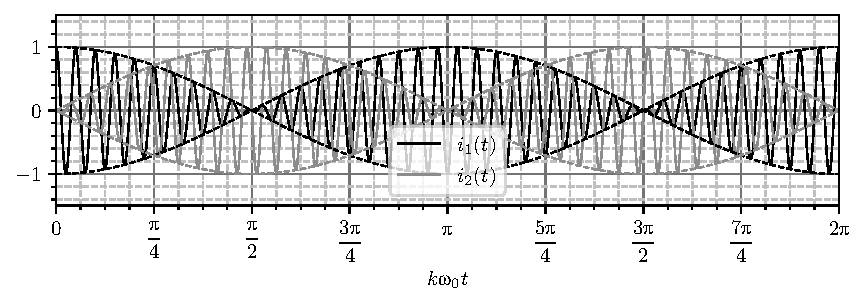
\includegraphics[scale=1]{fig/LC_plot.pdf}
    \caption{Илустрација резултата.}
    \label{fig:\ID.2}
\end{figure}

(в) Уколико се по претпоставци усвоји да је $k\ll1$ онда се може 
апроксимирати\footnote{Користи се апроксимација првим чланом Тејлоровог развоја
$(1 + x)^{\upalpha} \approx 1 + \upalpha x$, за $\upalpha = -\dfrac{1}{2}$.}
да је $\dfrac{1}{\sqrt{1 \pm k}} = 1 \mp \dfrac{1}{2}k$. Погоднији облик струја се може добити 
изражавањем збира, односно разлике косинуса преко производа.
\footnote{ Одговарајући тригонометријски идентитети јесу
$\cos x + \cos y = 2 \cos\left(\dfrac{x+y}{2}\right)\cos\left(\dfrac{x-y}{2}\right)$, 
и $\cos x - \cos y = - \sin\left(\dfrac{x+y}{2}\right)\sin\left(\dfrac{x-y}{2}\right)$} има се приближни
резултат:
\begin{eqnarray}
    & i_1(t) \approx I_0 \cos(2\upomega_0 t) \cos( k\upomega_0 t ), \\
    & i_2(t) \approx -I_0 \sin(2\upomega_0 t) \sin( k\upomega_0 t ).
\end{eqnarray}
Добијени резултати приказани су на графику на слици \ref{fig:\ID.2}. На слици пуном линијом 
су приказани одговарајући сигнали. Испрекиданим линијама приказане су анвелопе тих сигнала, 
које илуструју процес „шетања“ енергије између једног и другог осцилаторног кола. 
Појава која је добијена дешава се у општем случају у систему спрегнутих осцилатора. 



\vspace*{\ProblemSep}
\subsection{Преносне функције LTI система}

\refstepcounter{ID}
\setcounter{fid}{0}
\graphicspath{{./4_laplasova_transformacija/3_fje_prenosa/}}
\noindent
\newpage
\begin{slikaDesno}[0.83]{fig/tram.pdf}
    \textbf{\ID.} 
На слици \ID.1 приказан је упрошћени модел 
електричног трамваја масе $m = 20\unit{t}$ који
се креће по равној прузи. Трамвај 
се напаја из мреже константног напона $V_{\rm S} = 
650\unit{V}$. Мотор трамваја се представља 
идеалним струјним генератором, струје 
$i_{\rm g} = i_{\rm g}(t)$, која се 
може контролисати. Претпоставити да се сва снага
коју мрежа предаје мотору, без губитака, претвара у механичку 
енергију посредством механичке силе. 
На трамвај делује и сила отпора ваздуха
дата изразом ${\bf F}_{\rm ov} = -b {\bf v}$, где је\linebreak 
\vspace*{-3mm}
\end{slikaDesno} 
$b = 150\unit{\dfrac{N}{km/h}}$ a 
$v = v(t)$ је брзина трамваја.
Посматрамо систем чији једини
улаз представља струја $i_{\rm g}$ а једини
излаз тренутна брзина $v$ трамваја. 
Ако је познато да се тај систем може представити 
као каскадна веза једног линеарног система 
чија је функција преноса $H(s)$ и једног 
нелинеарног система без меморије чија је 
статичка преносна карактеристика $f(u)$,
одредити једно решење за 
$H(s)$ и $f(u)$. Објаснити да ли 
је посматрани систем линеаран.
Скицирати временски дијаграм тренутне брзине 
трамваја ако је управљачка струја дата изразом
$i_{\rm g} = I_0 \operatorname{rect}
\left( \dfrac{t}{T} - 1 \right)$,
где су $I_0 = 250\unit{A}$ и $T = 20\unit{s}$,
а трамвај полази из мировања.
\vspace*{1mm}

\noindent
\textit{\underline{Помоћ.}} Снага механичке силе $F$ која 
делује на круто тело које се креће брзином $v$ 
равна је $P = Fv$. \\

\textsc{\underline{Решење}}: (а) Укупна механичка снага која делује на трамвај разлика је снаге 
коју улаже генератор и снаге губитака на отпор ваздуха, 
\begin{equation}
P_{\rm meh} = P_{\rm g} - P_{\rm ov}. \label{eq:\ID.1}
\end{equation}
Снагом генератора се управља индиректно помоћу управљачке
струје, $P_{\rm g} = V_{\rm S} i_{\rm g}$ док је снага губитака на рачун отпора ваздуха 
$P_{\rm ov } = F_{\rm ov} v = -bv^2$. Пошто се трамвај креће по равној прузи механички рад 
претвара се у кинетичку енергију па је
$P_{\rm meh} = \dfrac{\de W_{\rm k}}{\de t} = \dfrac{m}{2} \dfrac{\de (v^2)}{\de t}$. Заменом 
свих одређених снага у израз добија се диференцијална једначина \eqref{eq:\ID.1}:
\begin{equation}
    \dfrac{m}{2} \dfrac{\de (v^2)}{\de t} =
    V_{\rm S} i_{\rm g} - bv^2
\end{equation}
%
\begin{figure}[b!]
    \centering
    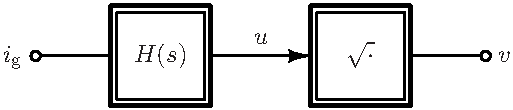
\includegraphics[scale=1]{fig/tram_diag.pdf}
    \caption{}
\end{figure}
%
Добијена диференцијална једначина по $v$ није линеарна, али се може приметити да је линеарна по $v^2$ што 
користимо увођењем одговарајуће смене $u = v^2$, чиме се добија диференцијална једначина  
на основу које се лако може наћи преносна функција $H(s) = \dfrac{U(s)}{I_{\rm g}(s)}$ \vspace*{1mm} као 
\begin{equation}
    \dfrac{m}{2} \dfrac{\de u}{\de t} =
    V_{\rm S} i_{\rm g} - bu \bigg|_{\mathcal L} \Rightarrow
    \dfrac{sm}{2} U(s) = V_S I_{\rm g}(s) - b U(s) \Rightarrow 
    H(s) = \dfrac{V_{\rm S}}{ \dfrac{m}{2} s + b }
\end{equation}
Одговарајућа смена се може третирати као нелинеарни систем без меморије, па је тако у целини 
дати систем представљен каскадном везом линеарног система функције преноса $H(s)$ и нелинеарног система
без меморије статичке преносне карактеристике $f(u) = \sqrt{u}$ као на слици \ID.2.

(б) Линеарност система проверава се испитивањем хомогености и адитивности. Систем је хомоген уколико, вреди 
$O\{kx(t)\} = kO\{x(t)\}$. Посматраћемо брзину у устаљеном стању, односно када је 
$\dfrac{\de v^2}{\de t} \to 0$, тада важи да је $V_{\rm S} i_{\rm g}(\infty) - bv(\infty)^2 \to 0$, односно 
$v(\infty) = \sqrt{\dfrac{V_{\rm S} i_{\rm g}(\infty)}{b}}$. На основу израза се види да је 
$v(\infty) \propto i_{\rm g}(\infty)$ па систем није хомоген, а самим тим ни линеаран. 
Нагласимо да у општем случају каскадна веза линеарног 
и нелинеарног система није линеаран систем, ипак, постоје практичне примене у којима се користе нелинеарни системи за изградњу система
који су у целини линеарни (нпр. транслинеарна кола у аналогној електроници).


\begin{figure}[b!]
    \centering
    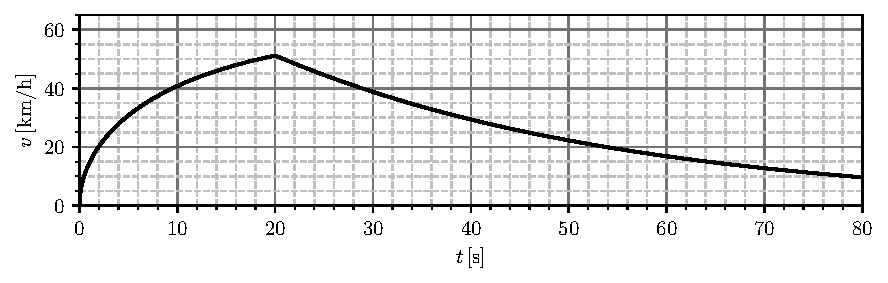
\includegraphics[scale=1]{fig/tram_plot.pdf}
    \caption{}
\end{figure}

    (в) Одзив на задату побуду одредићемо одређивањем међурешења $u(t)$. Побуда се може записати у облику 
    $i_{\rm g} = I_0 (u(t) - u(t - T))$. Тако да ће одзив бити 
    $u(t) = I_0 (g(t) - g(t - T))$, где је $g(t)$ одскочни одзив система $H(s)$, због његове линеарности. 
    Одскочни одзив одређујемо у комплексном домену, растављањем на парцијалне разломке
    \begin{align}
        G(s) = \underbrace{\dfrac{1}{s}}_{\LT{\uu(t)}} \cdot \underbrace{\dfrac{V_{\rm S}}{ \dfrac{m}{2} s + b } }_{H(s)}
        = \dfrac{A}{s} + \dfrac{B}{\dfrac{m}{2} s + b} 
        = 
        \begin{cases}
            A =  \dfrac{V_{\rm S}}{ \xcancel{s}\left( \dfrac{m}{2} s + b\right) } \bigg|_{s = 0} = \dfrac{V_{\rm S}}{b} \\
            B =  \dfrac{V_{\rm S}}{ {s} \,\, \xcancel{\left( \dfrac{m}{2} s + b\right) } } \bigg|_{s = -\frac{2b}{m}} = 
            -\dfrac{m V_{\rm S}}{2b}
        \end{cases}
    \end{align}
    Сређивањем добијеног израза добија се 
    $
    G(s) = \dfrac{V_{\rm s}}{b} \left( \dfrac{1}{s} - \dfrac{1}{s + \frac{2b}{m}} \right)$ \vspace*{1mm} 
    па се инверзном Лапласовом трансформацијом налази
    $g(t) = \mathcal{L}^{-1} \{ G(s) \} = \dfrac{V_{\rm S}}{b} \left(1 - \ee^{ -\frac{2b}{m} t } \right) \uu(t) $, 
    сређивањем се даље налази
    \begin{equation}
    u(t) = \dfrac{I_0 V_{\rm S}}{b} \Biggl(
        \left(1 - \ee^{ -\frac{2b}{m} t } \right) \uu(t) 
        -
        \left(1 - \ee^{ -\frac{2b}{m} (t - T)} \right) \uu(t - T),
    \Biggr)
    \end{equation}
    што се може расписати и као 
    \begin{eqnarray}
        u(t) = \dfrac{I_0 V_{\rm S}}{b} \cdot 
        \begin{cases}
            0 , & t < 0 \\
            1 - \ee^{-\frac{2b}{m}t} , & 0 < t < T \\
            ( \ee^{2bT/m} - 1) \ee^{-\frac{2b}{m}t} , & t > T 
        \end{cases}
    \end{eqnarray}
    па је израз за брзину са израчуатим константама: 
    \begin{eqnarray}
        v(t) \approx 62,5 \unit{\dfrac{km}{h}} \cdot 
        \sqrt{
        \begin{cases}
            0 , & t < 0 \\
            1 - \ee^{-t/18\unit{s}} , & 0 < t < T \\
            2,04\, \ee^{-t/18\unit{s}} , & t > T 
        \end{cases}
        }
    \end{eqnarray} 
    Добијени резултат приказан је на слици.




    

\vspace*{\ProblemSep}
\section{Одабирање и реконструкција сигнала}
\subsection{„Памти-прати“ (SH) кола}

\refstepcounter{ID}
\setcounter{fid}{0}
\graphicspath{{./5_odabiranje/1_kola/}}
\noindent
\begin{slikaDesno}{fig/SH_kolo.pdf}
\PID Сигнал $x(t) = 2\sin\left( \upomega_0 t\right)$,
где је $\upomega_0 = 100\uppi$, доводи се на улаз кола са слике. Прекидач у колу је отворен, осим у 
тренуцима $t = kT$ када је \textit{краткотрајно} затворен ($k \in \mathbb Z$). 
Познато је $T = \dfrac{2\uppi}{\upomega_{\rm s}}$, $\upomega_{\rm s} = 800\uppi$.
Ако се излазни сигнал кола, $x_{\rm s}(t)$ 
обради идеалним филтром функције преноса $H(\jj\upomega) = 
a \rect\left(\dfrac{\upomega}{4\upomega_0} \right)$, 
израчунати константу $a$ тако да се као резулат добије тачно 
$y(t) = \sin\left( \upomega_0 t + \upphi \right)$, и том приликом израчунати угао $0 \leq \upphi < 2\uppi$.
\end{slikaDesno} \\


\textsc{\underline{Решење}}: Операциони појачавачи у колу повезани су у конфигурацију два јединична 
бафера. Сигнал на излазу левог операционог појачавача једнак је сигналу $x(t)$, 
док је напон на кондензатору једнак напону на излазу кола $x_{\rm s}(t)$. Када је прекидач отворен, 
напон кондензатора се не мења, док при краткотрајном затварању у тренуцима $kT$, напон кондензатора 
прима вредност $x(kT)$. Ово доводи до степеничастог напона, израђеног од низа правоугаоних импулса.

\begin{figure}[hb!]
    \begin{subfigure}[t]{0.35\textwidth}
        \centering
        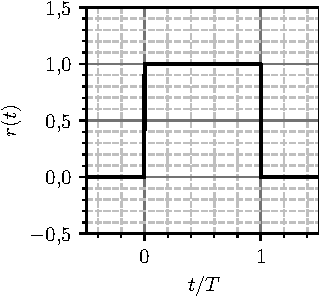
\includegraphics[scale=1]{fig/SH_plot_2.pdf}
        \caption{$r(t)$}        
        \label{fig:\ID.pulse}
    \end{subfigure}
    \hfill
    \begin{subfigure}[t]{0.55\textwidth}
        \centering
        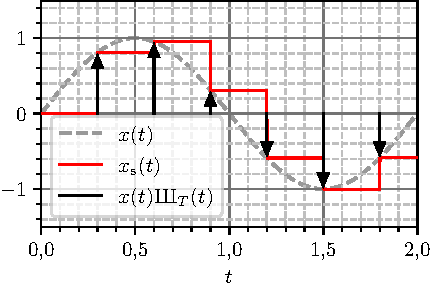
\includegraphics[scale=1]{fig/SH_plot_1.pdf}
        \caption{Уз пример, $T = 0,3$.}        
        \label{fig:\ID.primer}
    \end{subfigure}
    \caption{}
\end{figure}

Такав сигнал се може изградити помоћу низа померених правоугаоних јединичних импулса 
облика ${r(t) = \uu(t) - \uu(t - T)}$,
приказаних на слици \ref{fig:\ID.pulse}. Облик излазног сигнала се онда може представити као 
$x_{\rm s}(t) = \sum_{k = -\infty}^{\infty} x(kT) \cdot r(t - kT)$. Пошто се онда
конволуција са Дираковим импулсом може користити за померање у времену, односно важи
$r(t - kT) = r(t) \ast \updelta(t - kT)$, добијени израз се може трансформисати 
поступком\footnote{Користи се правило еквиваленције 
$x(kT) \updelta(t - kT) = x(t) \updelta(t - kT)$. }
  
\begin{equation}
x_{\rm s}(t) = \sum_{k = -\infty}^{\infty} x(kT) \cdot r(t - kT)    
             = \sum_{k = -\infty}^{\infty} x(kT) \cdot r(t) \ast \updelta(t - kT) = 
             r(t) \ast x(t) \III_T(t).  
\end{equation}

Тако добијени израз даје основу за фреквенцијску анализу сигнала. Одређивањем спектра 
таквог сигнала, применом теорема о трансформацији конволуције и проивода, налазимо резултат:

\begin{eqnarray}
    X_{\rm s}(\jj\upomega) = \mathcal{FT}\{ x_{\rm s}(t) \}
    = R(\jj\upomega) \cdot \dfrac{1}{\cancel{2\uppi}} 
    \left(X(\jj\upomega) \ast 
    \underbrace{\dfrac{\cancel{2\uppi}}{T}}_{\upomega_0} \III_{\upomega_s}(\upomega) \right)
    =
    \dfrac{1}{T}
    R(\jj\upomega) \sum_{k = -\infty}^{\infty} X(\jj(\upomega - k\upomega_s)) \nonumber \\
\end{eqnarray}

Излаз након филтрирања идеаалним филтром је онда облика 
$X_{\rm s}^{\text{(f)}}(\jj\upomega) = 
X_{\rm s}(\jj\upomega)\cdot H(\jj\upomega) = \dfrac{1}{T} R(\jj\upomega)
\sum_{k = -\infty}^{\infty} X(\jj(\upomega - k\upomega_s)) 
\cdot a \rect\left(\dfrac{\upomega}{4\upomega_0} \right)$. Пошто је задовољена 
теорема одбарињања ($\upomega_{\rm s} > 2\upomega_{0}$) не долази до преклапања спектралних реплика, 
па тако идеални филтар који одбацује све чланове ван опсега 
$\left(-\dfrac{\upomega_0}{2}, \dfrac{\upomega_0}{2}\right)$ задржава само централну 
спектралну реплику, за $k = 0$, тиме остаје резултат филтрирања
$X_{\rm s}^{\text{(f)}}(\jj\upomega) = 
X_{\rm s}(\jj\upomega)\cdot H(\jj\upomega)$, односно 
$
    X_{\rm s}(\jj\upomega) = \dfrac{a}{T} R(\jj\upomega)  X(\jj(\upomega)).
$
Практично, може се сматрати да се цео систем од улаза до излаза, у општијем случају 
под претпоставком задовољења теореме одабирања, може представити једном фунцкијом преноса 
облика 
\begin{equation}
    G(\jj\upomega) = \dfrac{X_{\rm s}^{\text{(f)}}}{X(\jj\upomega)} = \dfrac{a R(\jj\upomega)}{T}. \label{eq:\ID.general}
\end{equation}


Заменом резултата за спектар датог правогаоног импулса из задатка \ref{ID:rect_pulse_spectrum}
и спректра простопериодичног сигнала налазимо конкретан резултат за функцију преноса 
${G(\jj\upomega) = a \cdot \dfrac{1 - \ee^{-\jj\upomega T} }{\jj\upomega T}}$. Одређивањем функције преноса на учестаности
побуде $\upomega = \upomega_0$ налазе се појачање амплитуде и фазни померај излазног сигнала.  
\begin{align}
    |G(\jj\upomega_0)| = &\ a \left| \dfrac{1 - \ee^{-\jj\upomega T} }{\jj\upomega T} \right| = 
    \dfrac{ a\sqrt{2\bigl(1 - \cos(\upomega_0 T)\bigr)} }{\upomega_0 T} \\
    \arg G(\jj\upomega_0) = & \dfrac{\upomega_0 T - \uppi}{2} 
\end{align}
Пошто је према услову задатка $\upomega_0 T = \dfrac{\uppi}{4}$ коначно се добија да је 
$|G(\jj\upomega_0)| = \dfrac{4a}{\uppi} \sqrt{2 - \sqrt {2}}$ и $\upphi = -\dfrac{3\uppi}{8}$. Према услову задатка, 
амплитуда побудног и одзивног сигнала је иста, то мора бити $|G(\jj\upomega_0)| = 1$ па је 
$a = \dfrac{\uppi} { 4 \sqrt{2 - \sqrt {2}} }$.

Скренимо пажњу на општи закључак. Уколико је теорема одабирања задовољена, односно, уколико не долази до преклапања 
спектралних реплика, онда се резултат \ref{eq:\ID.general} може сматрати општим. Односно, он показује како облик 
реконструкционог импулса $r(t)$, утиче на спектар одзивног сигнала. 

Читаоцу се препоручује
да размотри какав се сигнал јавља на излазу целог система, уколико се уместо датог идеалног филтра 
пропусника ниских учестаности, $H(\jj\upomega)$ искористи филтар пропусник опсега учестаности, централне кружне учестаности $2 \upomega_0$. 

\vspace*{\ProblemSep}
\section{$\mathcal{Z}$--траснсформација}
\subsection{Системи диференцних једначина}

\refstepcounter{ID}
\setcounter{fid}{0}
\graphicspath{{./6_z_transformacija/2_sistemi/}}
\noindent
\newpage
\begin{slikaDesno}{fig/bouncing_blocks.pdf}
\textbf{{\color{red}*}\ID.}
    У механичком систему са слике познат
је однос 
маса крутих блокова $
\upalpha = \dfrac{M}{m}$. 
Зид са леве је веома масиван и 
практично непокретан, a са десне стране подлога 
се протеже у бесконачност.
Занемарити трење између подлоге 
и блокова, 
$\upmu \to 0$. 
У почетном тренутку су вектори брзина 
блокова
${\bf v} = v_0 {\rm i}_x$ и
${\bf u} = 0$ ($v_0 > 0$). 
\end{slikaDesno}
Након $k$ међусобних судара блокова су 
њихови алгебарски интензитети брзина 
$v[k]$ и $u[k]$.
% Нацртати (а) 
% блок дијаграм система, без улаза, 
% користећи идеалне блокове за кашњење, сабираче
% и множаче, тако да су његови излази буду 
% $v[n]$ 
% и $u[n]$, 
% барем до тренутка када 
% више нема судара у систему. 
(а) Одредити низове $v[k]$ и $u[k]$.
Одредити (б) укупан
број судара између блокова у процесу, $N$, 
ако је $\upalpha = 400^m$, где је $m$ цео број.
Сматрати да су сви судари у систему 
\textit{апсолутно еластични}. 

\textit{\myul{Помоћ}}. Након 
апсолутно еластичног
судара, дуж правца, између блокова масе $m_1$ и $m_2$ 
почетних алгебарских интензитета брзина $u_1$ и 
$u_2$ њихови нови алгебарски интензитети брзина су 
$v_1 = \dfrac{m_1-m_2}{m_1+m_2} u_1 + 
\dfrac{2m_2}{m_1+m_2} u_2$  и 
$v_2 = 
\dfrac{2 m_1}{m_1+m_2} u_1
+
\dfrac{m_2 - m_1}{m_1 + m_2} u_2  
$ редом. Референтни смерови брзина блокова 
су \myul{један ка другом}. \\

\textsc{\underline{Решење}}: Пошто се судари дешавају у дискретним временским тренуцима 
док је између њих стање система непроменљиво, процес представљен у задатку се може сматрати
\textit{дискретним} у односу на текући број судара. Стање након $k$-тог судара описано је
системом датих диференцних једначина као 
\begin{eqnarray}
    v[k+1] & = & \dfrac{M - m}{M + m} v[k] + \dfrac{2m}{M + m} (-u[k]) \\[2mm]
    u[k+1] & = & \dfrac{2M}{M + m} v[k] + \dfrac{m - M}{M + m} (-u[k]),
\end{eqnarray} 
Важно је нагласити да се у једначинама појављује $-u[k]$ будући да леви блок у судару учествује 
\textit{након} одбијања о зид са леве стране што доводи до промене знака брзине тог блока. 
Елиминисањем конкретних маса преко задатог параметра $\upalpha$ има се
\begin{eqnarray}
    v[k+1] & = & \dfrac{\upalpha - 1}{\upalpha + 1} v[k] - \dfrac{2}{\upalpha + 1} u[k] \\[2mm]
    u[k+1] & = & \dfrac{2\upalpha}{\upalpha + 1} v[k] - \dfrac{1 - \upalpha}{\upalpha + 1} u[k]
\end{eqnarray} 

%(а)

(б) Одређивање одзива система обавља се применом $\mathcal{Z}$-трансформације уз уважавање почетних 
услова\footnote{Користи се теорема $\mathcal Z\{x[n + 1]\} = z(\mathcal Z \{x[n]\} - x[0])$. }
чиме се добија
\begin{eqnarray}
    z(V(z) - 
    \cancelto{v_0}{v[0]}
    ) & = & \dfrac{\upalpha - 1}{\upalpha + 1} V(z) - \dfrac{2}{\upalpha + 1} U(z) \\[2mm]
    z(U(z) - \cancel{u[0]} ) & = & \dfrac{2\upalpha}{\upalpha + 1} V(z) - \dfrac{1 - \upalpha}{\upalpha + 1} U(z)
\end{eqnarray}
Сређивањем израза у форму система алгебарских једначина по $V(z)$ и $U(z)$ има се.
\begin{eqnarray}
    - z v[0] & = & \left( \dfrac{\upalpha - 1}{\upalpha + 1} - z \right) V(z) - \dfrac{2}{\upalpha + 1} U(z) \\[2mm]
    0 & = & \dfrac{2\upalpha}{\upalpha + 1} V(z) - \left( \dfrac{1 - \upalpha}{\upalpha + 1} + z \right) 
    U(z)
\end{eqnarray}
Решавањем система једначина налазе се резултати: 
\begin{eqnarray}
    U(z) & = & 
    \frac{2 \alpha v_{0} z}
    {z^{2} + 2 z \dfrac{1 - \upalpha}{1 + \upalpha} + 1}
    \\[2mm]
    V(z) & = & 
    \frac{v_{0} z \left(z + \dfrac{1 - \upalpha}{1 + \upalpha} \right) }
    {z^{2} + 2 z \dfrac{1 - \upalpha}{1 + \upalpha} + 1}
\end{eqnarray}
Непосредном идентификацијом, одређујемо инверзну $\mathcal{Z}$-трансформацију добијених резултата: 
$u[k] = v_0\sqrt\upalpha \sin(k\Upomega_0)$ и 
$v[k] = v_0\cos(k\Upomega_0)$, где је $\Upomega_0 = \arccos\left( \dfrac{\upalpha-1}{\upalpha+1} \right)$.

\begin{figure}[b!]
    \centering
    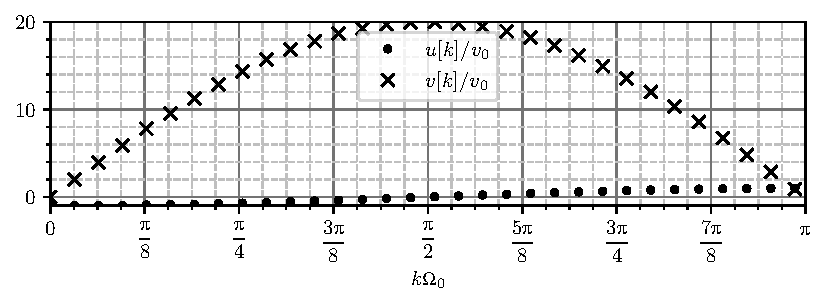
\includegraphics[scale=1]{fig/blokovi_plot.pdf}
    \caption{Пример за $\upalpha = 400$, укупно $N = \lfloor 10\uppi \rfloor = 31$ судара.}
    \label{fig:\ID.primer}
\end{figure}

Блокови ће наставити сударање све док након $k$ судара брзина десног блока у десно не постане
већа од брзине левог блока -- односно, када након одбијања левог блока о зид он не буде могао да 
сустигне већи блок. То је изражено условом у облику $- v[k] \geq u[k]$.  Гранично решење потражимо
у скупу реалних бројева сменом $k \mapsto t$ као
\begin{eqnarray}
    - \cancel{v_0} \cos(t\Upomega_0) & = & \cancel{v_0} \sqrt{\upalpha} \sin(t\Upomega_0)
    \Rightarrow
    \cos(t\Upomega_0) = -\sqrt{\upalpha} \sin(t\Upomega_0) \Rightarrow 
    \tan(t\Upomega_0) = -\dfrac{1}{\sqrt{\upalpha}}
    \\
    & \Rightarrow & t = \dfrac{1}{\Upomega_0} 
    \left( \arctan\left(-\dfrac1{\sqrt{\upalpha}} \right) + \uppi \right)
    \\
    & \Rightarrow & k_\mr{max} = N = \lfloor t \rfloor = \left\lfloor \dfrac{1}{\Upomega_0} \left( \arctan\left(
        -\dfrac1{\sqrt{\upalpha}} \right) + \uppi \right) \right\rfloor
        \label{eq:\ID.collisions}
\end{eqnarray}

Размотримо шта се дешава када $\upalpha$ постаје велико. Тада је 
$\arctan \left(- \dfrac1{\sqrt{\upalpha}} \right) 
\to 0$, a добијена дискретна кружна учестаност се може апроксимирати у околини јединице
помоћу Тејлоровог развоја\footnote{Када је $x\to 0$ тада је $\arccos(1 - x) \approx \sqrt{2x}$} поступком
\begin{equation}
    \Upomega_0 = \arccos\left( \dfrac{\upalpha-1}{\upalpha+1} \right)
    = \arccos\left( 1 - \dfrac{2}{\upalpha+1} \right)
    \approx \dfrac{2}{\sqrt{ \upalpha }}
\end{equation}
Заменом добијене апроксимације у израз \ref{eq:\ID.collisions} добија се резултат:
$N = \left\lfloor \uppi \sqrt{\upalpha}/2 \right\rfloor$. \vspace{1mm} 
Односно, уколико је $\upalpha = 400^m$ онда је 
$N = \left\lfloor 10^m \uppi \right\rfloor$, дакле, првих $m$ цифара броја $\uppi$ (!)
На слици \ref{fig:\ID.primer} приказан је један пример сигнала $v[k]$ и $u[k]$ за 
$\upalpha = 400$. 

\vspace*{\ProblemSep}
\appendix
\appendix
\graphicspath{{./100_appendix/}}
\counterwithin{figure}{chapter}
\counterwithin{equation}{chapter}
\chapter{Решавање диференцних једначина}


\section{Увод}
Диференцне једначине су једначине које су дефинисане
над бројевним низовима $x[n]$ ($n \in \mathbb N$).
Називају се још и \textit{рекурентним једначинама} 
будући да дају везу између $n$-тог члана и
преосталих чланова низа (рекурентна/рекурзивна веза).
У том смислу, диференцна једначина $k$-тог реда
је, на пример, једначина облика:
\begin{equation}
\Upphi( x[n], x[n-1], \ldots, x[n-k] ) = 0.
\end{equation}
Еквивалентно, овакве једначине могу се формулисати и дефинисањем 
текућег у односу на претходне и наредне чланове низа. 
Додатно, за јединствено решење диференцне једначине 
$k$-тог реда потребно је познавати $k$ вредности 
низа, на пример. $x[0], x[-1], \ldots, x[-k+1]$
(тзв. помоћне вредности) што 
је еквивалентно почетним условима диференцијалних 
једначина.
Решења диференцне једначине се у општем случају не 
налазе једноставно (налик на диференцијалне једначине).
Ипак, постоји поступак решавања за конкретан облик диференцних једначина погодан за примену у анализи линеарних система о коме ће бити речи и у овом 
документу. 

Најједноставнија диференцна једначина је једначина 
\begin{equation}
x[n] = kx[n-1],
\end{equation}
где је $k \in \mathbb R$ позната 
константа. Уколико усвојимо да је 
$x[0] = a$ лако се уочава шема:
\begin{eqnarray}
x[1] &=& kx[0] = ka \\
x[2] &=& kx[1] = k\cdot ka = k^2 a \\
x[3] &=& kx[2] = k\cdot k^2a = k^3 a \\
\vdots
\end{eqnarray} 
Односно, уочава се да је решење $x[n] = k^n a$. 
Практично, 
на основу формулације такве диференцне једначине 
поставља се као природно решење скалирана експоненцијална
функција $x[n] = Ck^n$. Ово је слично као у случају
диференцијалних једначина где су природна решења 
облика ${\rm e}^{\uplambda x}$. У оба случаја, заједничко
је то да под трансформацијом која дефинише једначину
(у случају диференцијалне једначине то је извод, а у
случају диференцне једначине то је \textit{кашњење}) 
природно решење \textit{не мења облик}:
\begin{eqnarray}
 e^{\uplambda t} 
\xrightarrow{\frac{{\rm d}}{{\rm d}t}}& 
\uplambda e^{\uplambda t} &\sim  {\rm e}^{\uplambda t} \\
\uplambda^{n} \xrightarrow{n\mapsto n-1}&
\uplambda^{n-1} = \dfrac{1}{\uplambda} \uplambda^{n} 
&\sim \uplambda^n 
\end{eqnarray}
Односно, као што решења линеарних диференцијалних 
једначина треба тражити у облику ${\rm e}^{\uplambda x}$
тако решења линеарних диференцних једначина треба 
тражити у облику $\uplambda^n$. 

\section{Линеарне хомогене диференцне једначине са
константним коефицијентима}

Обична линеарна хомогена диференцна једначина $k$-тог 
реда са константним реалним коефицијентима је једначина облика: 
\begin{equation}
 a_k x[n] + a_{k-1} x[n-1] + a_{k-2} x[n-2] + 
 \ldots a_0 x[n-k] = 0, \qquad (a_j \in \mathbb R)
 \label{de2}
\end{equation}
или у еквивалентном облику 
\begin{equation}
 a_k x[n+k] + a_{k-1} x[n+k-1] + \ldots a_0 x[n] = 0
 \qquad (a_j \in \mathbb R)
 \label{lhm}
\end{equation}
Где је  познато $k$ вредности за $x[n]$. 
Претпостављајући облик решења у облику
$x[n] = \uplambda^n$ и заменом у 
\eqref{lhm} има се: 
\begin{eqnarray}
& a_k \uplambda^{n+k} + 
a_{k-1} \uplambda^{n+k-1} + 
\ldots
+ a_0 \uplambda^n = 0 \, \Rightarrow \\ 
&
\uplambda^n(
a_k \uplambda^{k} + 
a_{k-1} \uplambda^{k-1} + 
\ldots
+ a_0) = 0. \label{P}
\end{eqnarray}
Члан у загради у изразу \eqref{P} назива се 
\textit{карактеристичним полиномом} диференцне једначине:
\begin{equation}
P(\uplambda) =
a_k \uplambda^{k} + 
a_{k-1} \uplambda^{k-1} + 
\ldots
+ a_0
\end{equation}
Добијени полином је исти и за другу варијанту 
диференцне једначине као из израза \eqref{de2}.
Степен полинома одговара реду диференцне једначине 
${\rm deg}\,P = k$, и једнак је броју линеарно независних
партикуларних решења диференцне једначине. 
Зависно од структуре скупа коренова овог полинома
$\{\uplambda_1, \uplambda_2, \ldots, \uplambda_k\}$ 
одређују се и сама партикуларна решења полазне 
диференцне једначине. Пошто је посматрана диференцна
једначина линеарна, њено опште решење јесте 
свака линеарна комбинација њених партикуларних
решења, односно:
\begin{equation}
x[n] = C_1 \uplambda_1^n + C_2 \uplambda_2^n + \cdots
+ C_k \uplambda_k^n.
\end{equation}
Уколико су неки од коренова вишеструки, јасно је онда
да сви чланови $\uplambda_i^n$ нису линеарно независни. На пример, 
уколико је $\uplambda_i = \uplambda_j$ онда је  
$C_i \uplambda_i + C_j \uplambda_j = (C_i + C_j) 
\uplambda_i$ само једно партикуларно решење. Показује
се да је друго партикуларно решење у том случају 
$n\uplambda_i^n$, односно, двоструком корену 
карактеристичног полинома $\uplambda_i$ одговарају
два партикуларна решења $\uplambda_i^n$ и 
$n\uplambda_i^n$. У општем случају корена $\uplambda_i$ вишеструкости $q$ њему одговарају $q$ партикуларних
решења и то $\{\uplambda_i^n, n\uplambda_i^n, 
n^2\uplambda_i^n, \ldots, n^{q-1}\uplambda_i^n\}$. 

Будући да су разматрани коефицијенти карактеристичног
полинома реални, то његови евентуално комплексни корени  
$\underline{\uplambda}_i = \uprho {\rm e}^{{\rm j}\upphi}$ морају имати комплексно 
конјуговани пар $\underline{\uplambda}_j=\underline{\uplambda}_i^* 
= \uprho {\rm e}^{-{\rm j}\upphi}$. Овим двома 
комплексним коренима одговарају и два линеарно независна
партикуларна решења диференцне једначине и то су 
$\underline{\uplambda}_i^n$ и 
${\underline{\uplambda}_i^*}^n$. То се 
може записати и на следећи начин, применом тригонометријског облика комплексног 
броја:
%\begin{eqnarray}\setlength{\mathindent}{0pt}
\begin{align}
C_i \underline{\uplambda}_i^n
+ C_j {\underline{\uplambda}_i^*}^n =& 
C_i \uprho^n(\cos(n\upphi) + 
{\rm j}\sin(n\upphi)) 
+ C_j \uprho^n(\cos(n\upphi) - 
{\rm j}\sin(n\upphi)) \\
=& \underbrace{(C_i + C_j)}_{\underline C_i'} \uprho^n \cos(n\upphi) + 
\underbrace{ {\rm j}(C_i - C_j)}_{\underline C_j'}\uprho^n \sin(n\upphi) \label{recttrig}
\end{align}
%\end{eqnarray}
Дакле, као еквивалентан пар линеарно независних 
решења могу се посматрати и $\{\uprho^n \cos(n\upphi), 
\uprho^n \sin(n\upphi)\}$. На сличан начин, 
множењем са $n^i$, се 
могу добити и партикуларна решења за вишеструке 
комплексно конјуговане полове као у претходном случају.

\subsection{Резиме} 
За једначине облика \eqref{lhm} или 
\eqref{de2} дефинише се карактеристични полином 
\eqref{P} чији скуп коренова одређује партикуларна 
решења према обрасцу:
\begin{itemize}
\item Сваком једноструком реалном корену $\uplambda_i$ 
одговара тачно једно партикуларно решење $\uplambda_i^n$.
\item Сваком вишеструком реалном корену $\uplambda_i$ 
вишеструкости $q$ одговара тачно $q$ партикуларних 
решења $\{\uplambda_i^n, n\uplambda_i^n, 
n^2\uplambda_i^n, \ldots, n^{q-1}\uplambda_i^n\}$
\item Сваком пару комплексно конјугованих коренова 
$\underline\uplambda_i$ и $\underline\uplambda_j 
= \underline\uplambda_i^*$ одговарају два партикуларна
решења и то $\{\uprho^n \cos(n\upphi), 
\uprho^n \sin(n\upphi)\}$.
\item Сваком пару вишеструкости $p$ комплексно конјугованих коренова 
$\underline\uplambda_i$ и $\underline\uplambda_j 
= \underline\uplambda_i^*$ одговарају $2p$
партикуларних
решења и то 
$$\{\uprho^n \cos(n\upphi), 
n\uprho^n \cos(n\upphi), 
n^2\uprho^n \cos(n\upphi), 
\ldots,
n^{p-1}\uprho^n \cos(n\upphi), 
\},$$
и
$$\{\uprho^n \sin(n\upphi), 
n\uprho^n \sin(n\upphi), 
n^2\uprho^n \sin(n\upphi), \ldots,
n^{p-1}\uprho^n \sin(n\upphi), 
\}.$$
\end{itemize}
тиме је исцрпљен скуп могућности за коренове 
карактеристичног полинома. Имајући свих $k$ 
линеарно независних партикуларних решења 
$x_{{\rm p},i}[n]$
има се коначно опште решење диференцне једначине у 
облику:
\begin{equation}
x[n] = C_1 x_{{\rm p},1}[n] +
 C_2 x_{{\rm p},2}[n] + \cdots + C_k x_{{\rm p},k}[n].
\end{equation}

\subsection{Примери}
\noindent
\textbf{Пример 1.} Одредити решење диференцне једначине 
\begin{equation}
x[n] - 4x[n-1] + 5x[n-2] - 4x[n-3]  + 4x[n-4] = 0
\end{equation}
ако су познате помоћне вредности $x[0] = 0$, 
$x[1] = 1$, $x[2] = 11$, $x[3] = 41$. \\[2mm]
\textbf{\underline{Решење}:} Карактеристични полином 
је $P(\uplambda) = \uplambda^4 - 4 \uplambda^3 
+ 5 \uplambda^2 - 4\uplambda + 4$. Коренове полинома степена већег од два 
у општем случају није лако наћи. Ипак, постоје неке 
препоруке 
за „погађање“ корена. На пример, уколико су сви корени 
целобројни, онда 
морају делити слободни члан. Дакле, потенцијални кандидати за целобројне 
корене су у овом случају $\{1,\,-1,\,2,\,-2,\,4,\,-4\}$. 
Лако се 
проверава да су $P(1) = 1$, $P(-1) = 18$,  
{$P(2) = 0$}, $P(-2) = 80$, $P(4) = 68$, $P(-4)=612$. 
Односно, један од коренова је 2. Да би се пронашли остали
корени, потребно је полином поделити са $(\uplambda - 2)$ 
што се може извести на више начина а најефикаснији је 
применом Хорнерове шеме: \\[2mm]
%
\begin{tabular}{c|cccccl}
& $\uplambda^4$ & $\uplambda^3$ & $\uplambda^2$
& $\uplambda^1$ & 1 \\ \hline \hline
& 1 & -4 & 5 & -4 & 4 \\
\boxed{2} & 1 & -2 & 1 & -2 & & $\Rightarrow 
\uplambda^3 - 2\uplambda^2 + \uplambda - 2$
\end{tabular}\\[2mm]

\noindent
Поново се утврђује провером да је целобројни корен овог 
полинома 2, односно, поступак треба поновити још једном:
\\[2mm]
\begin{tabular}{c|cccccl}
& $\uplambda^3$ & $\uplambda^2$ & $\uplambda^1$
& 1 \\ \hline \hline
& 1 & -2  & 1 & -2 \\
\boxed{2} & 1 & 0 & 1 & & $\Rightarrow 
\uplambda^2 + 1$
\end{tabular}\\[2mm]
Преостали су још само корени 
полинома $\uplambda^2 + 1$ што су $\{{\rm j}, -{\rm j}\}$.


Коначно, сви корени карактеристичног полинома су
$[2,2,{\rm j},-{\rm j}]$. Двоструком корену 
$\uplambda_1 = 2$ одговарају два партикуларна решења
и то $x_{\rm p,1}[n] = 2^n$ и $x_{\rm p,2}[n] = n 2^n$.
Конјугованом пару $\{{\rm j}, -{\rm j}\}$ одговарају 
два партикуларна решења. 
$\left\{ 
\cos\left( 
\dfrac{n\uppi}{2}
\right),
\sin\left( 
\dfrac{n\uppi}{2}
\right)
\right\}
$
Опште решење је облика:
\begin{equation}
x[n] = C_1 2^n + C_2 n2^n + C_3
\cos\left( 
\dfrac{n\uppi}{2}
\right)
+ C_4
\sin\left( 
\dfrac{n\uppi}{2}
\right)
\end{equation}
Заменом помоћних вредности у добијено опште решење 
добија се систем једначина:
\begin{equation}
\begin{aligned}
x[0] &= 0 = \, C_1 + C_3 \\
x[1] &= 1 = \, 2C_1 + 2C_2 + C_4 \\
x[2] &= 11 = \, 4C_1 + 8C_2 - C_3\\
x[3] &= 41 = \, 8C_1 + 24C_2 - C_4.
\end{aligned}
\end{equation}
Решавањем добијеног система једначина добијају се 
непознате константе 
$C_1 = -1$, $C_2 = 2$, $C_3 = 1$, $C_4 = -1$. Заменом
у опште решење и сређивањем добија се коначни резултат
\begin{equation}
x[n] = (2n - 1)2^n + \cos\left( 
\dfrac{n\uppi}{2}
\right)
-
\sin\left( 
\dfrac{n\uppi}{2}
\right)
\end{equation}
\begin{flushright}
$\blacksquare$
\end{flushright}

\noindent
\textbf{Пример 2.} Одредити решење диференцне једначине
\begin{equation}
x[n] + x[n-1] - x[n-2] - x[n-3] = 0
\end{equation}
које задовољава $x[0] = 2$, $x[1] = -1$ и 
$x[2] = 3$. \\[2mm]
\textbf{\underline{Решење}:} Карактеристични полином
је $P(\uplambda) = \uplambda^3 + \uplambda^2 
- \uplambda - 1$. Полином се може директно факторисати
\begin{align}
P(\uplambda) & = \uplambda^3 + \uplambda^2 
- \uplambda - 1 \\
& = \uplambda^2 (\uplambda + 1) 
- (\uplambda + 1) \\
& = (\uplambda^2 - 1) (\uplambda + 1) \\
& = (\uplambda - 1) (\uplambda + 1)^2. 
\end{align}
Такав карактеристични полином има корене 
$[1, -1, -1]$ на основу чега има опште решење: 
\begin{equation}
x[n] = C_1 + (C_2 + C_3 n) (-1)^n.
\end{equation}
Заменом помоћних вредности добија се систем 
једначина:
\begin{align*}
x[0] = 2 =&\, C_1 + C_2 \\
x[1] = -1 =&\, C_1 - C_2 - C_3 \\
x[2] = 3 =&\, C_1 + C_2 + 2C_3
\end{align*}
Решења овог система једначина су 
$C_1 = \dfrac{3}{4}$, $C_2 = \dfrac{5}{4}$, 
$C_3 = \dfrac{1}{2}$. Коначно решење примера је:
\begin{equation}
x[n] = \dfrac{3}{4} + \left( \dfrac{5}{4} + 
\dfrac{1}{2} n \right) (-1)^n
\end{equation}


\chapter{Операциони појачавач и индуктивни елементи}

\section{Напонски диференцијални појачавач}
Поједностављен модел реалног 
напонског 
диференцијалног појачавача без меморије, приказан на слици \ref{fig:da1}, карактерисан је својом улазном отпорношћу $R_{\rm u}$, 
излазном отпорношћу $R_{\rm i}$ и напонским појачањем $A$ напонски
контролисаног напонског генератора.  
%
\begin{figure}[ht!]
\centering
    \begin{subfigure}[c]{0.32\textwidth}
    \centering
        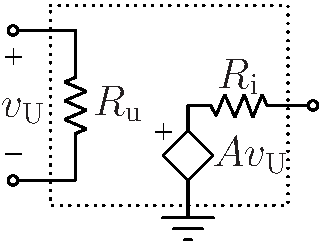
\includegraphics[scale=0.8]
        {fig/diff-amp.pdf}
        \caption{Унутрашња структура.}
        \label{fig:da1}
    \end{subfigure}
    %
    \begin{subfigure}[c]{0.32\textwidth}
    \centering
        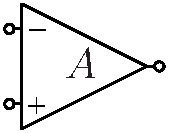
\includegraphics[scale=0.8]
        {fig/diff-amp-symb.pdf}
        \caption{Симбол.}
        \label{fig:da2}
    \end{subfigure}
\caption{Уз диференцијални појачавач}
\end{figure}
Има два улаза, један инвертујући 
(обележен са „-“) и један неинвертујући (обележен са „+“). Шематски симбол представљен је на 
слици \ref{fig:da2}.
Добар диференцијални напонски појачавач задовољава да су $R_{\rm u}\to\infty$, 
$R_{\rm i}\to0$. Такав диференцијални појачавач практично 
представља идеалан напоном контролисан напонски генератор, када је 
$v_{\rm I} = A v_{\rm U}$.

\section{Негативна повратна спрега}
\begin{figure}[b!]
    \centering
    \begin{subfigure}[c]{0.32\textwidth}
    \centering
        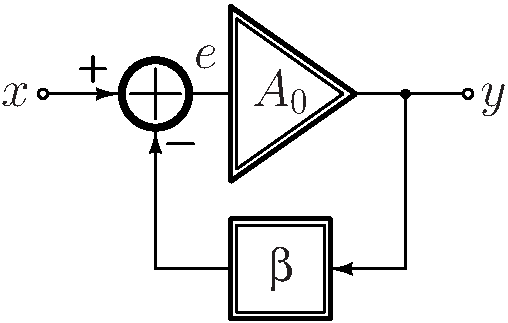
\includegraphics[scale=0.5]
        {fig/black-model.pdf}
        \caption{Блеков модел.}
        \label{fig:black}
    \end{subfigure}
    ~ %add desired spacing between images, e. g. ~, \quad, \qquad, \hfill etc. 
      %(or a blank line to force the subfigure onto a new line)
    \begin{subfigure}[c]{0.32\textwidth}
    \centering
        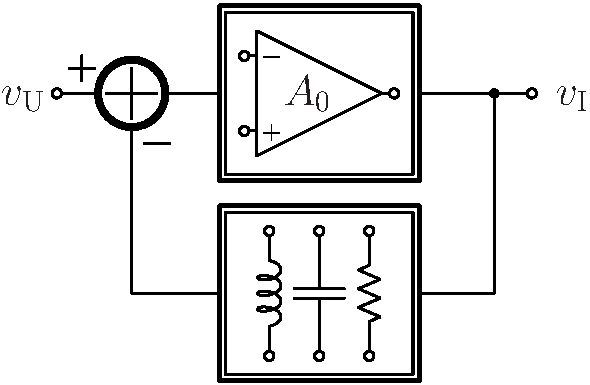
\includegraphics[scale=0.5]
        {fig/black-model-op.pdf}
        \caption{Блеков модел, са ОП.}
        \label{fig:op2}
    \end{subfigure}
    ~ %add desired spacing between images, e. g. ~, \quad, \qquad, \hfill etc. 
    %(or a blank line to force the subfigure onto a new line)
    \begin{subfigure}[c]{0.32\textwidth}
    \centering
        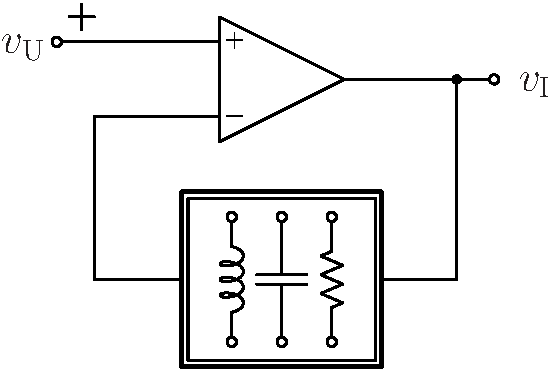
\includegraphics[scale=0.5]
        {fig/black-model-op-conc.pdf}
        \caption{Операциони појачавач, пример.}
        \label{fig:black3}
    \end{subfigure}
    \caption{Уз увођење принципа операционог појачавача.}
\end{figure}
%
Концепт који суштински мења начин употребе диференцијалног појачавача 
је са принцип реакције (повратне спреге). Блеков модел система са реакцијом 
приказан је 
блок дијаграмом
на слици \ref{fig:black}. У овом моделу, главни 
појачавач има појачање $A_0$ а мрежа повратне спреге појачање 
$\upbeta$. Појачање целокупног система се добија на основу 
блок дијаграма:
\begin{eqnarray}
	&e = x - \upbeta y \\
	&y = A_0 e, 
\end{eqnarray}
одакле се сређивањем добија појачање целог система
$A = \dfrac{y}{x} = \dfrac{A_0}{1 + \upbeta A_0}$.   
%
Сигнал $e$ назива се још и \textit{сигналом грешке}, а може се 
изразити преко улазног сигнала као $e = \dfrac{1}{1 + \upbeta A_0}x$.
Повратна спрега посебно добија на вредности када се размотри 
главни појачавач са веома великим појачањем, $A_{0} \to \infty$. У том случају су $A_{\infty} = \lim_{A_{0} \to \infty} 
\dfrac{A_0}{1 + \upbeta A_0} = \dfrac{1}{\upbeta}$ и 
$e_{\infty} = \lim_{A_{0} \to \infty} 
\dfrac{1}{1 + \upbeta A_0} = 0$. Односно, за довољно велико појачање 
главног појачавача, {карактеристике} {система са 
повратном спрегом диктира мрежа повратне спреге}. Посебно, ова топологија се 
може реализовати, на пример, помоћу операционог појачавача 
са пасивном мрежом повратне спреге, што је илустровано на слици 
\ref{fig:op2}. Према пређашњој дискусији, карактеристике оваквог 
система зависиће само од мреже повратне спреге ако је напонско 
појачање оваквог доброг диференцијалног појачавача веома велико. 
Такав диференцијални појачавач, 
ког кога је још и $A_0 \to \infty$, назива се \textbf{идеални 
операциони појачавач}. Идеални операциони појачавач најчешће 
обележавамо изостављањем ознаке 
напонског
појачања. Разлика улазног и повратног сигнала која се 
појачава, у ваљано одабраној топологији
(нпр. слика \ref{fig:black3}), 
мора бити разлика напона на улазима операционог појачавача, на основу чега
резултат да је $e_{\infty} \to 0$ повлачи 
то да се у оваквом режиму \myul{изједначавају напони инвертујућег
и неинвертујућег улаза}. Важно је нагласити, да ово није једина 
тополошка опција, већ да се улазни и излазни сигнал могу 
одузимати и на другачије начине, што се може видети на разним 
примерима (нпр. инвертујући појачавач). 
%
%

%
Коначно, уколико је операциони појачавач примењен у режиму 
повратне спреге онда се он може анализирати помоћу три правила која следе из пређашње анализе: \\

\shadowbox{
\begin{minipage}{0.5\textwidth}
\textbf{\myul{Идеалан операциони појачавач}}
\begin{itemize}
\item $i_+ = i_- = 0$ (јер је $R_{\rm u} \to 0$)
\item $v_+ = v_-$ (јер је $e_{\infty} \to 0$)
\item Излаз има произвољну вредност, тако да су 
задовољени пређашњи услови, $-\infty < v_{\rm OP} < \infty$.
\end{itemize}
\end{minipage}
%
\begin{minipage}{0.4\textwidth}
\begin{flushright}
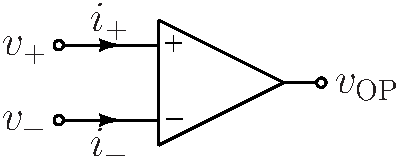
\includegraphics[scale=0.8]{fig/op.pdf}
\end{flushright}
\end{minipage}
}

\section{Индуктивни трансформатори}
\subsection{Спрегнути калемови}
Физички модел на коме су утемељени индуктивни трансформатори је модел 
спрегнутих калемова. Магнетска спрега два посматрана линеарна намотаја,
индуктивности $L_1$ и $L_2$ описује се
међусобном индуктивношћу $L_{\rm 12} = L_{\rm 21}$ (за реципрочне средине). Коефицијент магнетске спреге се дефинише као апсолутна 
вредност међусобне индуктивности сведена на јединицу геометријске
средине индуктивности појединих намотаја: 
$k = \dfrac{|L_{12}|}{\sqrt{L_1 L_2}}$, за знак међусобне 
индуктивности је одређен и смером мотања намотаја и шематски 
се обележава тачкама. Без додатних услова овакав пар спрегнутих 
калема описан је једначинама у временском домену:

\begin{center}
\shadowbox{
\begin{minipage}{0.3\textwidth}
\textbf{\myul{Пар спрегнутих калемова}}
\vspace*{0.5em}
\begin{itemize}
\item $v_1 = L_1 \dfrac{\de i_1}{\de t} + 
L_{12} \dfrac{\de i_2}{\de t}$ 
\item $v_2 = L_{12} \dfrac{\de i_1}{\de t} + 
L_{2} \dfrac{\de i_2}{\de t}$ 
\end{itemize}
\end{minipage}
%
\begin{minipage}{0.25\textwidth}
\begin{flushright}
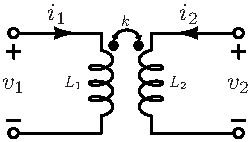
\includegraphics[scale=0.8]{fig/spregnuti.pdf}
\end{flushright}
\end{minipage}
}
\end{center}

За решавање проблема са спрегнутим калемовима, уколико су калемови 
кратко спојени са једне стране неретко је веома згодно прво обавити \textit{распрезање калемова} трансфигурацијом у еквивалентну
Т--мрежу као на слици \ref{raspreg}. Будући да је ово трансфигурација, 
то подразумева да су ове две мреже еквивалентне у сваком смислу.

\begin{figure}[ht!]
\centering
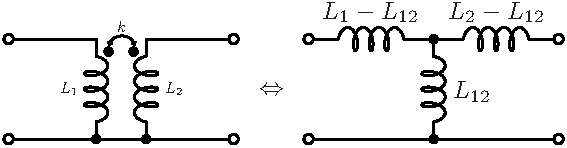
\includegraphics[scale=1]{fig/rasprezanje.pdf}
\caption{Уз распрезање калемова.}
\label{raspreg}
\end{figure}

\subsection{Савршени трансформатор}
Уколико је магнетска спрега трансформатора савршена, односно 
уколико нема магнетског расипања, $k = 1$, односно $L_{\rm 12} = \pm \sqrt{L_1 L_2}$,
такав трансформатор се назива \textbf{савршеним}. 
Без умањења  
општости, претпоставимо да су референтни смерови напона намотаја
одабрани тако да је $L_{\rm 12} = \sqrt{L_1 L_2}$. Тада се 
елиминацијом струја из модела спрегнутих калемова може показати да 
важи $\dfrac{v_1}{v_2 } = \sqrt[]{\dfrac{L_1}{L_2}}$. Пошто је 
сопствена индуктивност намотаја сразмерна квадрату броја навојака 
$L_i \propto N_i^2$, онда је и 
\begin{equation}
\boxed{
\dfrac{v_1}{N_1} = \dfrac{v_2}{N_2}
}
\end{equation}


\subsection{Идеални трансформатор}
Уколико посматрамо савршени трансформатор и за контуру средње 
линије језгра напишемо Уопштени Амперов закон имамо једначину 

\begin{equation}
N_1 i_1 + N_2 i_2 = \dfrac{B l}{\upmu_0 \upmu_r},
\label{uaz}
\end{equation}
где су 
$B$ интензитет вектора магнетске индукције у језгру, $l$ 
дужина средње линије језгра и $\upmu_{\rm r}$  релативна пермеабилност
материјала од кога је израђено језгро. Представимо број навојака оба намотаја нормализовано као $N_{i} = n_i N_0$ и заменимо у 
израз \eqref{uaz}. Тада $n_{i}$ представља релативни број 
навојака у односу на нормализациони фактор
$N_0$. За $N_0$ се може
одабрати, на пример, ред величине броја навојака оба намотаја. Уколико
су $N_1 = 1000$ и $N_2 = 2000$ онда се може одабрати на пример 
$n_1 = 1$ и $n_2 = 2$ за $N_0 = 1000$. Другим речима, са $n_i$ кодификујемо релативан број навојака намотаја а са $N_0$ њихов ред величине. Са тиме у виду 
једначину \eqref{uaz} можемо записати и као:
\begin{equation}
n_1 i_1 + n_2 i_2 = \dfrac{Bl}{\upmu_0 N_0 \upmu_r}
\end{equation}
Сада, приметимо да уколико је $\upmu_{\rm r}N_0 \to \infty$ онда 
једначина постаје $\boxed{n_1 i_1 + n_2 i_2 = 0}$. 
Тиме се добија модел \textbf{идеалног} 
трансформатора описан са две \textbf{алгебарске} једначине:

\noindent
\begin{center}
\shadowbox{
\begin{minipage}{0.3\textwidth}
\textbf{\myul{Идеални трансформатор}}
\vspace*{0.5em}
\begin{itemize}
\item $
\dfrac{v_1}{n_1} = \dfrac{v_2}{n_2}
$
\item $i_1 n_1 + i_2 n_2 = 0$ 
\end{itemize}
\end{minipage}
%
\begin{minipage}{0.25\textwidth}
\begin{flushright}
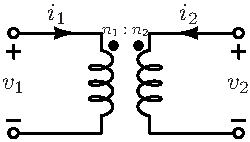
\includegraphics[scale=0.8]{fig/it-trafo.pdf}
\end{flushright}
\end{minipage}
}
\end{center}

\noindent
\begin{crtice}
Иако се 
материјал језгра при пројектовању 
може одабрати тако да $\upmu_{\rm r}$ буде велико, 
на пример трафо-лимови ($\upmu_{\rm r} \sim 100$), доступни материјали
постављају неку горњу границу пермеабилности. Са друге стране, инжењерским 
одабиром при пројектовању трансформатора може се одабрати велики 
број навојака намотаја тако да овај услов буде што боље задовољен.
На пример, уколико се пројектује трансформатор који треба да 
удвостручава напон, одабир $(N_1, N_2) = (200, 100)$ је бољи 
од одабира $(N_1, N_2) = (20, 10)$. To je углавном разлог 
зашто су скоро сви практични трансформатори са веома великим 
бројем намотаја, јер је често циљ направити што \textit{идеалнији}
трансформатор. 
Ипак, постоје и неки нарочити изузеци, као на пример Теслин 
трансформатор. 
За тачно одређивање потребног 
броја навојака постоје и други критеријуми, али ћемо се 
зауставити на овој илустрацији.
\end{crtice}

\subsection{Магнетизациона индуктивност}

Савршен трансформатор може се представити и помоћу 
идеалног трансформатора и једне индуктивности. Положај 
те индуктивности се 
може одабрати тако да се решавање кола 
највише поједностави
(са примарне или секундарне стране). Без доказа наводимо 
трансфигурацију: \\[0.5mm]
 
\noindent
\shadowbox{
\begin{minipage}{0.3\textwidth}
\textbf{\myul{Магнетизациона индуктивност}}
\\[0.5mm]
 
$L_{\rm m} = L_1$ \\[0.5mm]

$n = \sqrt{\dfrac{L_2}{L_1}}$
\end{minipage}
%
\begin{minipage}{0.7\textwidth}
\begin{flushright}
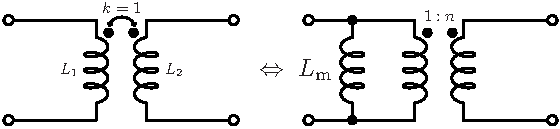
\includegraphics[scale=1]{fig/magnetizac.pdf}
\end{flushright}
\end{minipage}
}

Овај документ се надовезује на вежбе држане четврте 
седмице. Циљ документа је да обједини и појасни на примерима
методе за одређивање импулсног одзива континуалних 
\textit{LTI} система. 

\chapter{Одређивање импулсног одзива континуалних 
\textit{LTI} система} \label{a:impulsni_odziv}

\section{Поједностављење опште форме}

Посматрајмо континуални \textit{LTI} систем описан 
диференцијалном једначином облика
\begin{equation}
 P({\rm D}) y(t) = Q({\rm D}) x(t),
 \label{def}
\end{equation}
где су $x(t)$ и $y(t)$ побуда и одзив система редом, а  $P({\rm D})$ и $Q({\rm D})$ произвољни полиноми 
по оператору диференцирања $\rm D$. Импулсни  
одзив овог система $h = h(t)$ представља одзив система на 
јединичну импулсну
побуду $x(t) = \updelta(t)$, односно решење једначине
\begin{equation}
 P({\rm D}) h(t) = Q({\rm D}) \updelta(t).
 \label{phqd}
\end{equation}
Уколико приметимо смену 
\begin{equation}
\boxed{
 h(t) = Q({\rm D}) h_1(t)
} \label{hqh1}
\end{equation}
и заменимо у израз \eqref{phqd}, даље се може писати
\begin{equation}
P({\rm D}) h(t) = Q({\rm D}) \updelta(t) 
\enspace\Leftrightarrow\enspace
P({\rm D}) Q({\rm D}) h_1(t) = Q({\rm D}) \updelta(t) 
\enspace\Leftrightarrow\enspace
Q({\rm D}) P({\rm D}) h_1(t) = Q({\rm D}) \updelta(t). 
\end{equation}
У последњем кораку, начињена је замена редоследа 
примене оператора, $P({\rm D}) Q({\rm D})
\equiv Q({\rm D}) P({\rm D})$, која је 
оправдана на основу линеарности. У последњем 
кораку се може на обе стране применити оператор
$Q^{-1}({\rm D})$, чију егзистенцију овде нећемо
дискутовати, након чега преостаје резултат:
\begin{equation}
\boxed{
P({\rm D}) h_1(t) = \updelta(t). 
} \label{eq2}
\end{equation}

\noindent
\ovalbox{
\begin{minipage}{0.99\textwidth}
На основу претходно изнесеног поступка, могуће је 
одредити импулсни одзив система описаног једначином
\eqref{def} тако што се одреди помоћни одзив 
$h_1(t)$ помоћног система описаног једначином  
\eqref{eq2} a потом трансформацијом добијеног 
помоћног одзива у одзив полазног система помоћу 
\eqref{hqh1}
\end{minipage}
} 

\vspace*{2mm}
Додатно, из практичних 
разлога постоји ограничење у степенима
полинома $\deg P \geq \deg Q$.  
Уколико се импулсни одзив помоћног система запише 
у облику $h_1(t) = g(t)\,{\rm u}(t)$, онда се
могу разликовати случајеви:
\begin{equation}
h(t) = 
\left\{
\begin{array}{ll}
Q(D)\bigl( g(t){\rm u}(t) \bigr), & \deg P = \deg Q \\
Q(D)\bigl( g(t)\bigr)\, {\rm u}(t) , & \deg P > \deg Q \\
\end{array}
\right.
\end{equation}


\section{Одређивање импулсног одзива за
поједностављену форму}

На основу претходне дискусије, потребно је и довољно
одредити решење једначине 
$P({\rm D}) h_1(t) = \updelta(t)$. Препоручена 
метода
за решавање овог проблема је (\textit{i}) 
диференцирањем одскочног одзива (дискутовано на предавањима), али се може користити и 
(\textit{ii}) 
поједностављена
метода уклапања импулса (енг. 
\textit{impulse matching}, дискутовано на вежбама).
\\[1mm]
\indent
Прва метода утемељена је на својству линеарности 
система. Нека је $s_1(t) = O\{ {\rm u}(t) \}$ 
одскочни
одзив посматраног система, онда се диференцирањем 
обе стране изналази
\begin{equation}
\dfrac{{\rm d}s_1(t)}{{\rm d}t} = 
\dfrac{{\rm d}}{{\rm d}t} O\{ {\rm u}(t) \}
= 
 O\left\{ 
 \dfrac{{\rm d}}{{\rm d}t} {\rm u}(t) \right\}
 = O\{\updelta(t)\} = h_1(t),
\end{equation}
при чему је у другом кораку замењен редослед 
примене оператора диференцирања и система због
линеарности. Коначно се има закључак 
$
\boxed{
\dfrac{{\rm d}s_1(t)}{{\rm d}t} =  h_1(t)
},
$ 
односно, \textbf{импулсни одзив се добија диференцирањем  одскочног одзива}. Одређивање одскочног одзива 
представља решавање диференцијалне једначине 
$P({\rm D}) s_1(t) = {\rm u}(t)$. Велика предност 
у решавању на овај начин у односу на директно 
решавање једначине \eqref{eq2} јесте то да у њој 
\myul{нема импулса} што за последицу 
има то да је одскочни одзив непрекидан, тако да су
једнаке преиницијалне и постиницијалне вредности 
за $s_1(t)$. Будући да се одскочни одзив 
одређује за преиницијалне услове равне нули 
то повлачи да су онда и постиницијални услови 
равни нули. 
Одскочни одзив добија се као збир хомогеног и 
партикуларног дела $s_1 = s_{1\rm h} + s_{1\rm p}$. 
Хомогени део се одређује на начин показан на часу.
Партикуларни део
представља устаљени одзив на 
експоненцијалну побуду ${\rm e}^{0\cdot t} 
{\rm u}(t)$ и на основу дискусије са часа вежби 
једнак је $s_{\rm 1p} = \dfrac{1}{P(0)}$.
\\[1mm]
\indent
Друга метода утемељена је на особини линеарне 
независности различитих извода Диракових импулса.
%\begin{crtice} 
Може се показати да једначина облика:
\begin{equation}
a_0 \updelta(t) + 
a_1 \updelta'(t) + 
a_2 \updelta''(t) + 
\cdots
+ a_n \updelta^{(n)}(t) = 0, \quad (n \in \mathbb N)
\end{equation} 
по непознатим коефицијентима $a_0, a_1, 
\ldots, a_n \in \mathbb R$ има \myul{само} тривијално 
решење $a_0 = a_1 = a_2 = \cdots = a_n = 0$. 
У контексту решавања диференцијалне једначине 
облика $P({\rm D}) h_1(t) = \updelta(t)$ то значи да:
(\textit{i}) пошто се са десне стране налази делта 
импулс мора се налазити и са леве стране и 
(\textit{ii}) пошто се са десне стране не налазе 
изводи делта импулса њега не може бити ни са леве 
стране. На основу тога, у изразу 
$P({\rm D}) h_1(t)$ се мора појавити делта импулс
и не сме се појавити његов први извод. Претпоставимо 
да се сабирак $f(t) \updelta(t)$ јавља у $k$-том 
изводу импулсног одзива, $h_1^{(k)}(t)$, у том 
случају се у $(k+1)$-вом изводу импулсног 
одзива мора наћи сабирак облика 
$f'(t) \updelta(t) + {f(t) \updelta'(t)}$.
Односно, да се не би са леве стране појавио извод 
Дираковог импулса, неопходно је да се импулс 
појављује тек у највишем изводу импулсног одзива
који се јавља у једначини а то је $h^{(\deg P)}(t)$,
где је $\deg P$ степен полинома $P$ -- ред 
диференцијалне једначине. Будући да се импулс јавља
у $h^{(\deg P)}(t)$ то се Хевисајдова одскочна 
функција мора јављати у $h^{(\deg P - 1)}(t)$, односно
до прекида долази у $(\deg P - 1)$-вом изводу. Будући
да су интеграли Хевисајдове функције непрекидни, то 
је онда тај и једини извод импулсног одзива који  има 
прекид. На основу тога, ако распишемо 
оператор система као 
$P({\rm D}) = c_0 + c_1{\rm D} + c_2{\rm D}^2 + 
\cdots + c_2{\rm D}^n$ једначина се може писати као
\begin{eqnarray}
& (c_0 + c_1{\rm D} + c_2{\rm D}^2 + 
\cdots + c_2{\rm D}^n) h_1(t) = \updelta (t)  \\
& c_0 h_1(t) +
c_1 h_1'(t) +
c_2 h_1''(t) +
\cdots
+ c_n h_1^{(n)}(t)
  = \updelta (t)
\end{eqnarray}
Ако интегралимо обе стране добијене једначине
$\int_{-\upepsilon}^{+\upepsilon}$ у
произвољно „уским“ границама, $\upepsilon \to 0$, 
приметивши да онда интеграли свих ограничених функција
теже нули преостаје само члан са импулсом:
\begin{align} 
    \DS
&
\cancel{ \DS
c_0 \int_{-\upepsilon}^{+\upepsilon}h_1(t) \,\de t
} +
\cancel{ \DS
c_1 \int_{-\upepsilon}^{+\upepsilon}h_1'(t) \,\de t
} +
%c_2 
%\cancel{ \DS \int_{-\upepsilon}^{+\upepsilon}h_1''(t) \,\de t 
%} +
\cdots
+ c_{n-1}  
\cancel{ \DS \int_{-\upepsilon}^{+\upepsilon}h_1^{(n-1)}(t) \,\de t}
% } + c_n \int_{-\upepsilon}^{+\upepsilon} h_1^{(n)}(t) \,\de t 
  = 
\underbrace{  \DS
  \int_{-\upepsilon}^{+\upepsilon} \updelta (t)\,\de t
}_{=1, \text{по деф.}} \nonumber
\Rightarrow \\[-2mm]
& 
c_n h_1^{(n-1)}(0^+)
-
c_n h_1^{(n-1)}(0^-) = 1 
\end{align} 
Како су преиницијални услови приликом тражења
импулсног одзива равни нули то преостаје 
$h_1^{(n-1)}(0^+) = \dfrac{1}{c_n}$.
%\end{crtice}
\noindent
\textbf{Коначно су непосредно 
познати сви постиницијални услови импулсног одзива
}
\begin{equation}
\boxed{
h_1^{}(0^+) = 0,
\enspace h_1^{'}(0^+) = 0,
\enspace h_1^{''}(0^+) = 0,
\ldots, 
\enspace h_1^{(n-2)}(0^+) = 0,
\enspace h_1^{(n-1)}(0^+) = \dfrac{1}{c_n},
}
\end{equation}
где је $c_n$ коефицијент уз највиши извод у
диференцијалној једначини а $n$ је ред диференцијалне
једначине.

\vspace*{10mm}



\noindent\textbf{Пример 1.} Одредити одзив система 
описаног диференцијалном једначином 
$y''(t) + 3 y'(t) + 2y(t) = x'(t) + 2x(t) $, 
на побуду $x(t) = 2e^t\,{\rm u}(t-2)$. \\[1mm]
%

\noindent\textbf{Решење.} Одзив на дату побуду $x(t)$
може се одредити конволуцијом. За примену конволуције
потребно је прво одредити импулсни одзив система. 
Систем се може записати у облику \eqref{def} за
$P({\rm D}) = {\rm D}^2 + 3 {\rm D} + 2$ и 
$Q({\rm D}) = {\rm D} + 2$. Потражимо импулсни одзив
помоћног система $P({\rm D}) h_1(t) = \updelta(t)$.

%\begin{flushright}
%\begin{minipage}{0.9\textwidth}
\vspace*{2mm}
\noindent
\textbf{1. метода} (\textit{диференцирањем импулсног 
одзива}). Импулсни одзив помоћног система 
тражимо као решење једначине 
\begin{equation}
P({\rm D}) s_1(t) = {\rm u}(t).
\label{eq:step}
\end{equation} Импулсни одзив
има хомогени део одређен коренима полинома $P$ и то 
$\uplambda \in \{-2, -1\}$. Облик хомогеног решења 
је онда $s_{\rm 1,h} = C_1 {\rm e}^{-t} + C_2
{\rm e}^{-2t}$. Партикуларни део је 
$s_{\rm 1,p} = \dfrac{1}{P(0)} = \dfrac{1}{2}$. 
Коефицијенти у општем облику једначине одскочног одзива
%$
%s_1(t) = C_1 {\rm e}^{-t} + C_2
%{\rm e}^{-2t} + \dfrac{1}{2}
%$
налазе се на основу постиницијалних почетних услова 
који су из раније наведених разлога равни нули. 
\begin{eqnarray}
s_1(t) = C_1 {\rm e}^{-t} + C_2
{\rm e}^{-2t} + \dfrac{1}{2} \Rightarrow &
s_1(0) = 0 = C_1 + C_2 + \dfrac{1}{2} \\
s_1'(t) = -C_1 {\rm e}^{-t} - 2 C_2
{\rm e}^{-2t}  \Rightarrow &
s_1'(0) = 0 = -C_1 -2 C_2 .
\end{eqnarray}
Решавањем добијеног система једначина по 
непознатим коефицијентима добија се 
$C_1 = -1$, $C_2 = \dfrac{1}{2}$. Одакле се 
коначно налази одскочни одзив 
$
s_1(t) = 
\left(	
-{\rm e}^{-t} + \dfrac{1}{2}{\rm e}^{-2t} + 
\dfrac{1}{2} \right) {\rm u}(t).
$ 
Диференцирањем добијеног одскочног одзива 
добија се и импулсни одзив помоћног система
$
\boxed{
h_1(t) =
\left(
{\rm e}^{-t}  - {\rm e}^{-2t} 
\right) \, {\rm u}(t)
}
$

\vspace*{2mm}
\noindent
\textbf{2. метода} (\textit{поједностављеном
методом уклапања импулса}) Непосредно се решава 
једначина $P({\rm D}) h_1(t) = \updelta(t)$. 
Општи облик импулсног одзива одређен је коренима 
полинома $P$ на исти начин као у претходној 
методи,
$h_1(t) = C_1 {\rm e}^{-t} + C_2 {\rm e}^{-2t}$.
На основу закључка методе познати су постиницијални почетни 
услови као $h_1(0^+) = 0$, $h_1'(0^+) = 1$. 
Заменом у општи облик добија се:
\begin{eqnarray}
h_1(t) = C_1 {\rm e}^{-t} + C_2
{\rm e}^{-2t}  \Rightarrow &
h_1(0^+) = 0 = C_1 + C_2  \\
h_1'(t) = -C_1 {\rm e}^{-t} -2 C_2
{\rm e}^{-2t}  \Rightarrow &
h_1'(0^+) = 1 = -C_1 - 2 C_2,  \\
\end{eqnarray}
решавањем добијеног система имају се $C_1 = -C_2 = 1$,
одакле је $\boxed{
h_1(t) =
\left(
{\rm e}^{-t}  - {\rm e}^{-2t} 
\right) \, {\rm u}(t)
}$
%\end{minipage}
%\end{flushright}

\vspace*{5mm}
\noindent
Имајући импулсни одзив помоћног система, импулсни
одзив полазног система налази се на основу 
\eqref{hqh1}, одакле је 
\begin{equation}
h(t) = Q({\rm D}) h_1(t) \Rightarrow 
\boxed{ h(t) = 
{\rm e}^{-t}
 \,{\rm u}(t) }. \label{eq:hodh1}
\end{equation}
\noindent
Одзив на побуду може се потражити конволуцијом 
\begin{equation}
y_{\rm p}(t) = h(t) \ast x(t). \label{konv}
\end{equation} 
У овом случају
је најефикасније применити својства конволуције. 
Побудни сигнал се може записати и као
$x(t) = 2{\rm e}^{t {\color{blue} - 2 + 2}}
\,{\rm u}(t-2) = 2{\rm e}^2 {\rm e}^{t-2} {\rm u} (t-2)$.
Приметимо да је побудни сигнал временски померен 
и скалиран у односу на сигнал $x_1 = e^{t} \, {\rm u}(t)$. Да би се 
израчунала конволуција \eqref{konv} згодно је 
искористити ово својство тако да се конволуција 
одговарајућим трансформацијама своди на табличну, 
или једноставнију
конволуцију. На основу таблице је 
$y_{\rm p,1} = h(t) \ast x_1(t) = 
{\rm e}^{-t} {\rm u}(t) \ast {\rm e}^{t} {\rm u}(t)
= \dfrac{{\rm e}^t - {\rm e}^{-t} }{2} 
{\rm u}(t) = {\rm sinh}(t) \, {\rm u}(t).
$
На основу линеарности и временске инваријантности, 
пошто важи $x(t) = 
2{\rm e}^2 x_1(t - 2)$ то је и 
$y_{\rm p}(t) = 
2{\rm e}^2 y_{\rm p,1}(t - 2)$ одакле је 
\begin{equation}
\boxed{
\boxed{
y_{\rm p}(t) = 2{\rm e}^2 {\rm sinh}(t-2) \, {\rm u}(t-2)
}
}
\end{equation}
\begin{flushright}
$\blacksquare$
\end{flushright}

